\chapter{Statistical analysis and results}
\label{chap:statandresults}

The signal and background models described in \Chapter~\ref{chap:model} are used to perform the statistical interpretation of the 12.9\ifb of data, resulting in an independent observation of the Higgs boson in the diphoton decay channel and measurements of some of its properties. %The objective is to twofold: 

The statistical analysis proceeds in several stages. The first step is to determine the best signal-plus-background fit of the models to the data. The floating parameters of the signal and background models are varied simultaneously in each analysis category to obtain the closest overall agreement with the observed invariant mass distributions. This procedure is described in \Sec~\ref{sec:statandresults:bestfit}, and establishes the existence of a Higgs boson signal in the data. The next step is to formally quantify the significance of this signal, and to reject the hypothesis that there exists no Higgs boson. The procedure for hypothesis testing and calculation of the signifiance is detailed in \Sec~\ref{sec:statandresults:significance}. Having established the existence of a \SM-like Higgs boson which decays to photons, the final step is to make measurements of some of its properties, in particular those which relate to the rate at which it is produced or interacts with other \SM particles. These measurements are described in \Sec~\ref{sec:statandresults:sigstrength} and \Sec~\ref{sec:statandresults:kappas}. 
 
As with all Higgs boson analyses performed within the \CMS collaboration, the statistical interpretation uses the frequentist approach. The corresponding statistical tools and techniques are briefly explained as they are needed throughout this chapter.

\section{Best fit of models to the data}
\label{sec:statandresults:bestfit}

The observed \mgg distributions obtained from the data in each analysis category (labelled $ \mgg^{obs}$ hereafter) are parametrised with models consisting of signal and background components. The tool which is used to assess the agreement of the data and the model in a category $C$ is called the \emph{likelihood function},

\begin{equation}
\label{eq:statandresults:likelihood_function}
\mathcal{L}_C(\mu, \mH; \mathbf{n} | \mgg^{obs} ) = \mu \cdot f_S(\mgg^{obs} |\mH ; \mathbf{n}_S) + f_B(\mgg^{obs} | \mathbf{n}_B ), 
\end{equation}

where: 
\begin{itemize}
\item $\mathbf{n}$ is a set of floating nuisance parameters, composed of those which affect the signal and those which affect the background, labelled $\mathbf{n}_S$ and $\mathbf{n}_B$ respectively; 
\item $f_S$ and $f_B$ represent the normalised probability distribution functions of the signal and background components of the model respectively; 
\item $\mu = \sigma^{H} / \sigma^{H}_{SM}$ is a \POI called the signal strength, where in this context $\sigma^H$ is the observed Higgs boson cross section, and $\sigma^H_{SM}$ is the \SM \crosssection. 
\end{itemize}
The overall likelihood function $\mathcal{L}$ for the simultaneous fit of all categories at once is obtained by taking the product of the likelihood functions $\mathcal{L}_C$ in each analysis category, taking care the correlate the corresponding nuisance parameters in each one.

The construction of the signal component of the model, $f_S$, was described in \Sec~\ref{model:sec:signal_model}. When performing the signal-plus-background fit to the data, the values of the individual parameters of the signal model functional form are fixed. Specifically, since the \SSF method was used, this refers to the coefficients of the seventeen polynomial functions which describe the dependence on \mH of the \DCBpG parameters for each of the \RV and \WV scenarios and their mixing fraction. The parameters which are allowed to vary are the nuisance parameters  $\mathbf{n}_S$  introduced into the signal modelling to account for systematic uncertainties (see \Sec~\ref{model:sec:systematics}) as well as the \POI\s $\mu$ and \mH. The signal strength $\mu$ uniformly scales all the signal models for each process and for each category. This means that the contribution to the overall signal model from each process remains in proportion to what is predicted by the \SM, but the normalisation of the overall signal model can be varied. 

The handling of the background component of the model $f_B$ was described in \Sec~\ref{model:sec:background_model}. The nuisance parameters $\mathbf{n}_B$ in each category are composed of:
\begin{itemize}
\item the discrete nuisance parameter which corresponds to the choice of background function, as prescribed by the discrete profiling method (see \Sec~\ref{model:sec:background_model_envelope}); 
\item the individual parameters of all the candidate functions, which are allowed to float in the fit.
\end{itemize}

%The fit is obtained by minimising twice the negative log-likelihood ($ -2 \ln \mathcal{L}(\mu, \mH ; \mathbf{n}| \mgg^{obs}$) or \NLL). 
The fit is obtained by minimising twice the negative log-likelihood (\NLL). 
The best-fit values of the \POI\s and nuisance parameters are denoted as $\hat{\mu}$, $\hat{\mH}$ and $\hat{\mathbf{n}}$, and correspond to :
\begin{equation}
%(\hat{\mu}, \hat{\mH} , \hat{\mathbf{n}}) = 
\{ (\mu, \mH, \mathbf{n}) : -2 \ln \mathcal{L}(\hat{\mu}, \hat{\mH} ;\hat{\mathbf{n}}| \mgg^{obs}) = \inf _{\mu,\mH , \mathbf{n}}(-2 \ln \mathcal{L}(\mu, \mH; \mathbf{n}| \mgg^{obs})) \},
\end{equation}
where $\inf_{ \mu, \mH ,\mathbf{n}}$ represents the \emph{infimum function} evaluated over all allowed values of $\mu$, \mH and $\mathbf{n}$, taking into account their constraints. This technique can be generalised for an arbitrary number of \POI\s. In general, the \NLL cannot be minimized analytically. Instead, this task is handled numerically with the \Minuit package~\cite{minuit}. 

The resulting parametrisations of the observed data are shown for each analysis category separately in \Fig\s~\ref{fig:statandresults:s_b_fits} and~\ref{fig:statandresults:s_b_fits_bis}. The combined parametrisations and data  resulting from a direct sum of each category is shown in \Fig~\ref{fig:statandresults:s_b_fits_direct_sum}, while the sum weighted by the $S/(S+B)$ in $\pm \effSigma$ around the best-fit $\mH$ in each category is shown in \Fig~\ref{fig:statandresults:s_b_fits_s_sb_sum}. The best-fit values of the \POI\s are $\hat{\mu}= 0.95$ and $\hat{\mH}= 126.0\GeV$, indicating a strong \SM-like Higgs boson signal. 


\begin{figure}[hpt!]
\centering
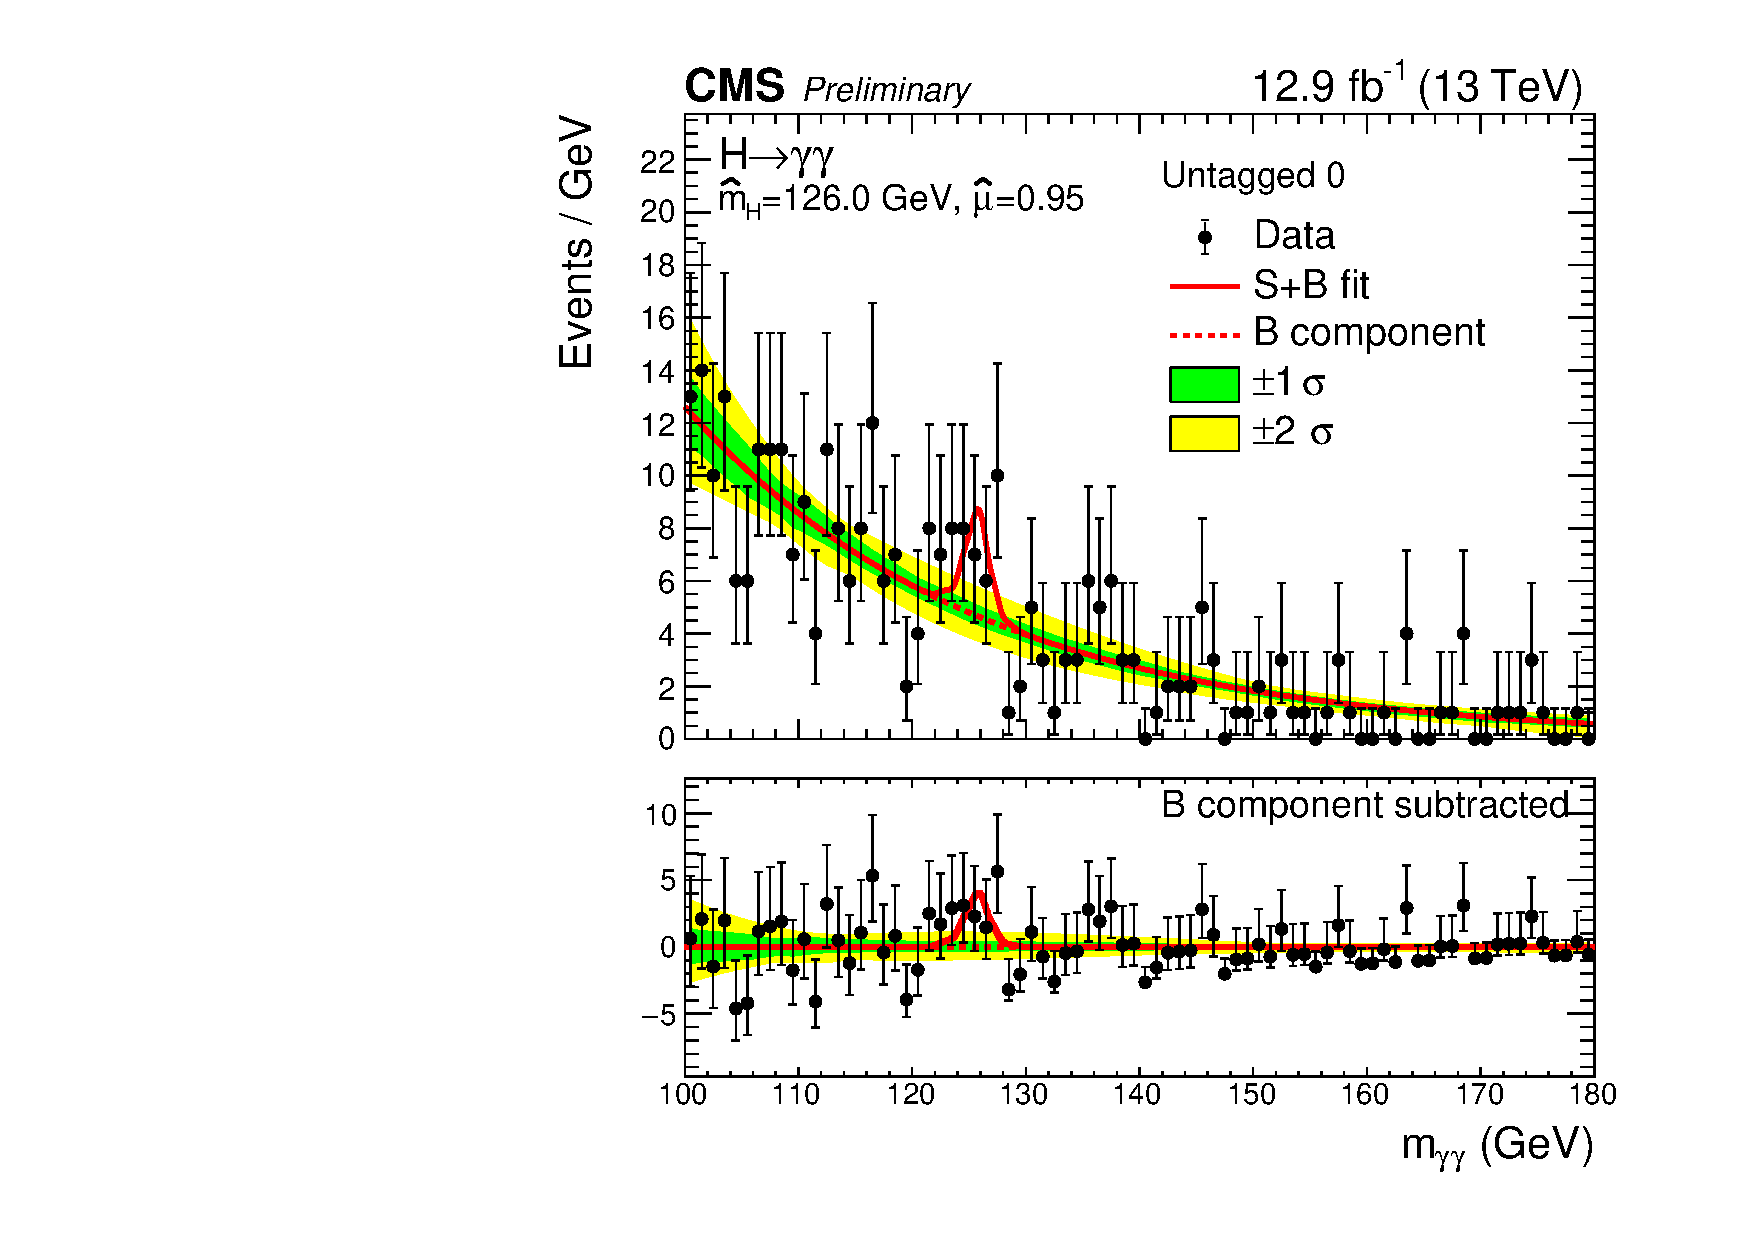
\includegraphics[width=0.49\textwidth]{statandresultsFigures/S_SB_ProfileMH_UntaggedTag_0_13TeV.pdf} 
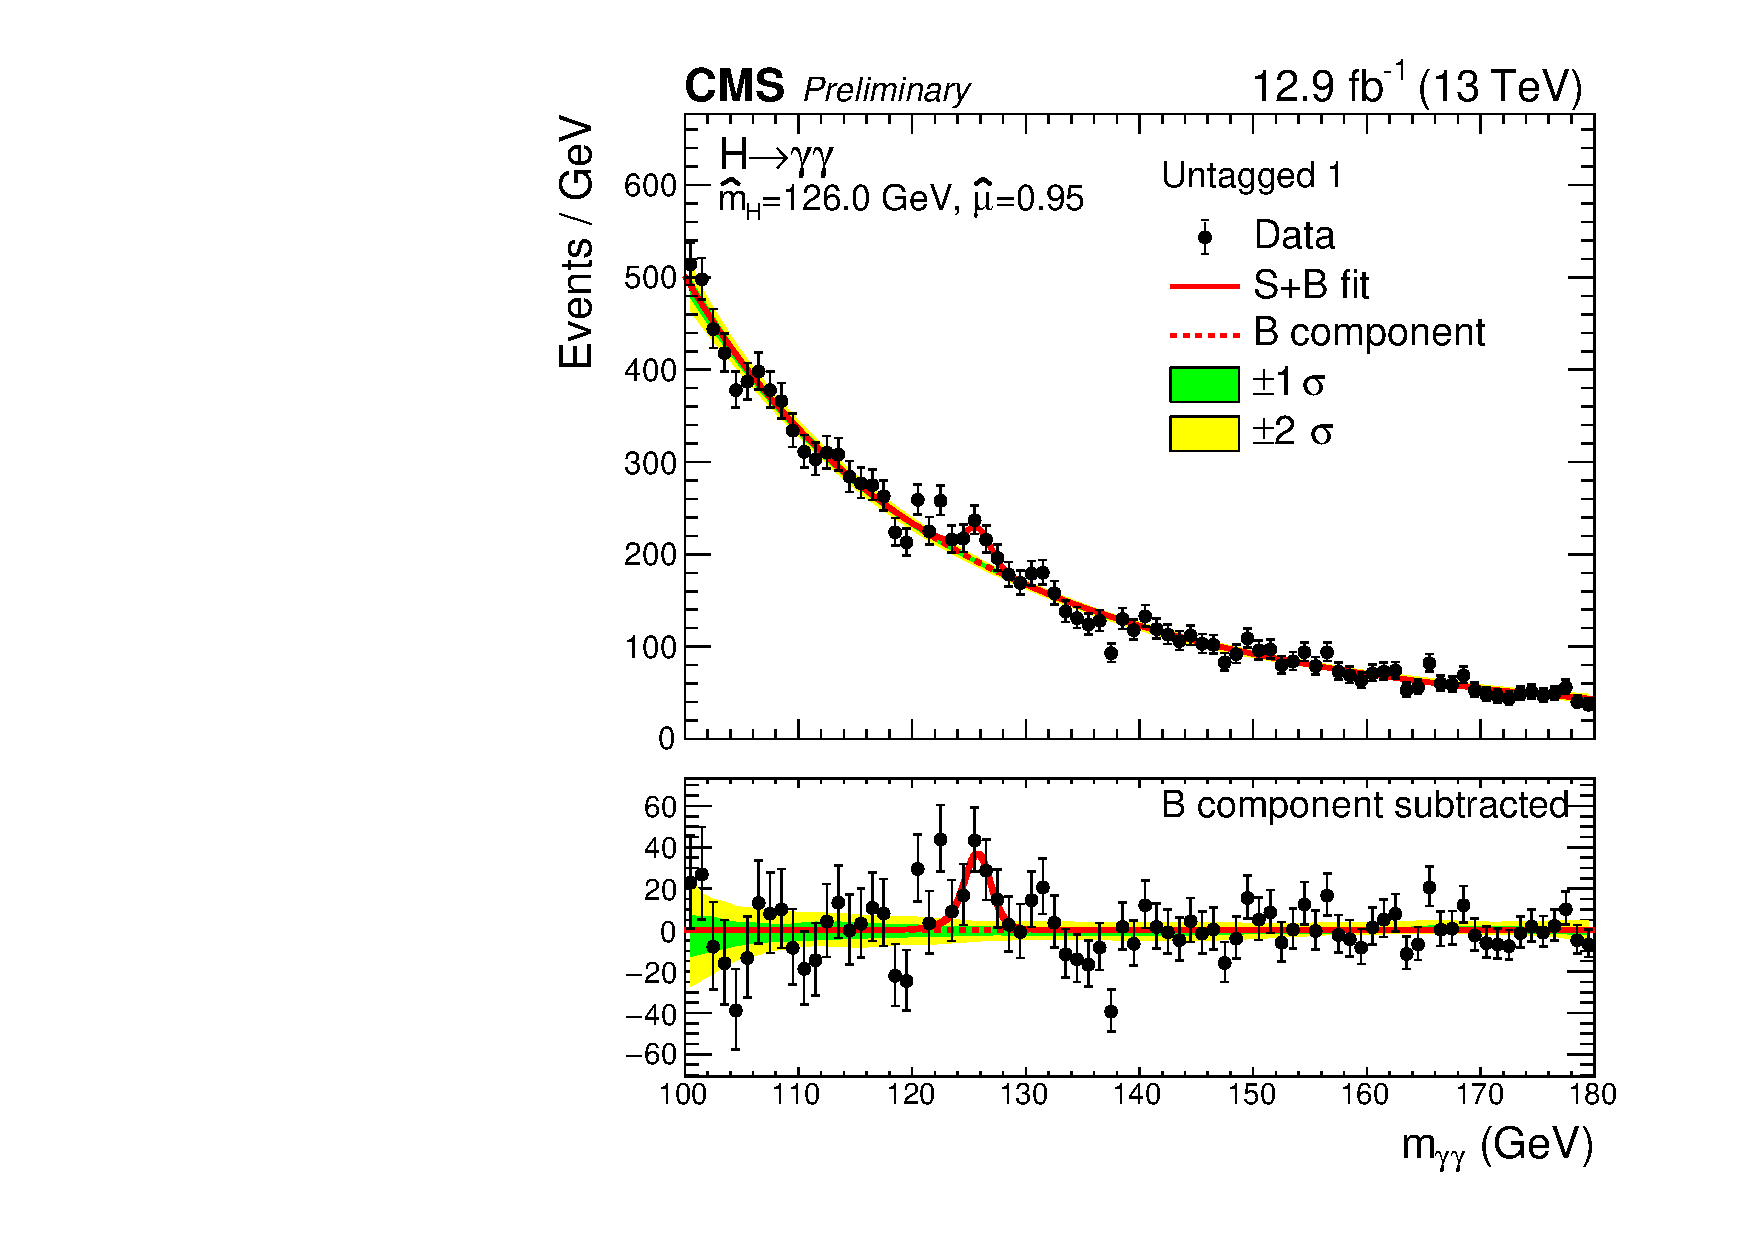
\includegraphics[width=0.49\textwidth]{statandresultsFigures/S_SB_ProfileMH_UntaggedTag_1_13TeV.pdf}\\ 
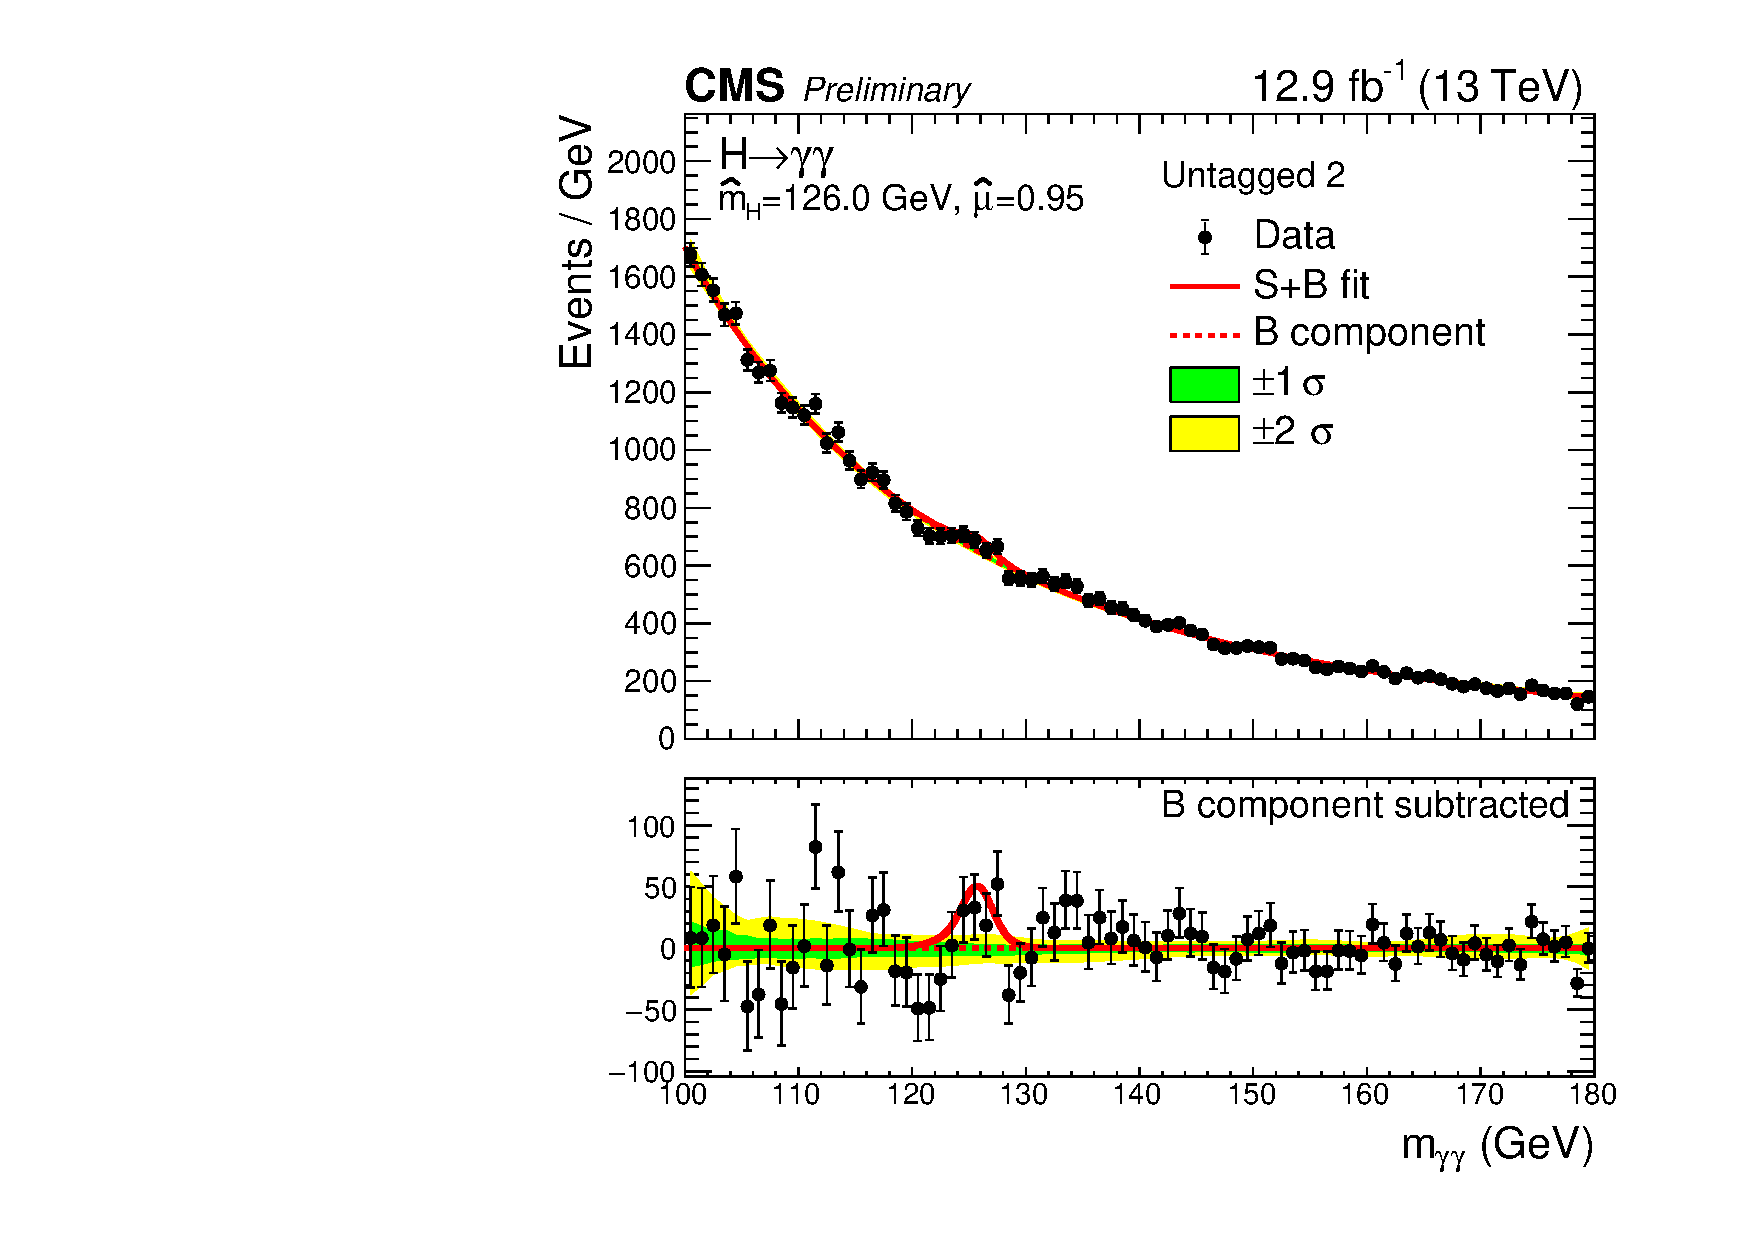
\includegraphics[width=0.49\textwidth]{statandresultsFigures/S_SB_ProfileMH_UntaggedTag_2_13TeV.pdf} 
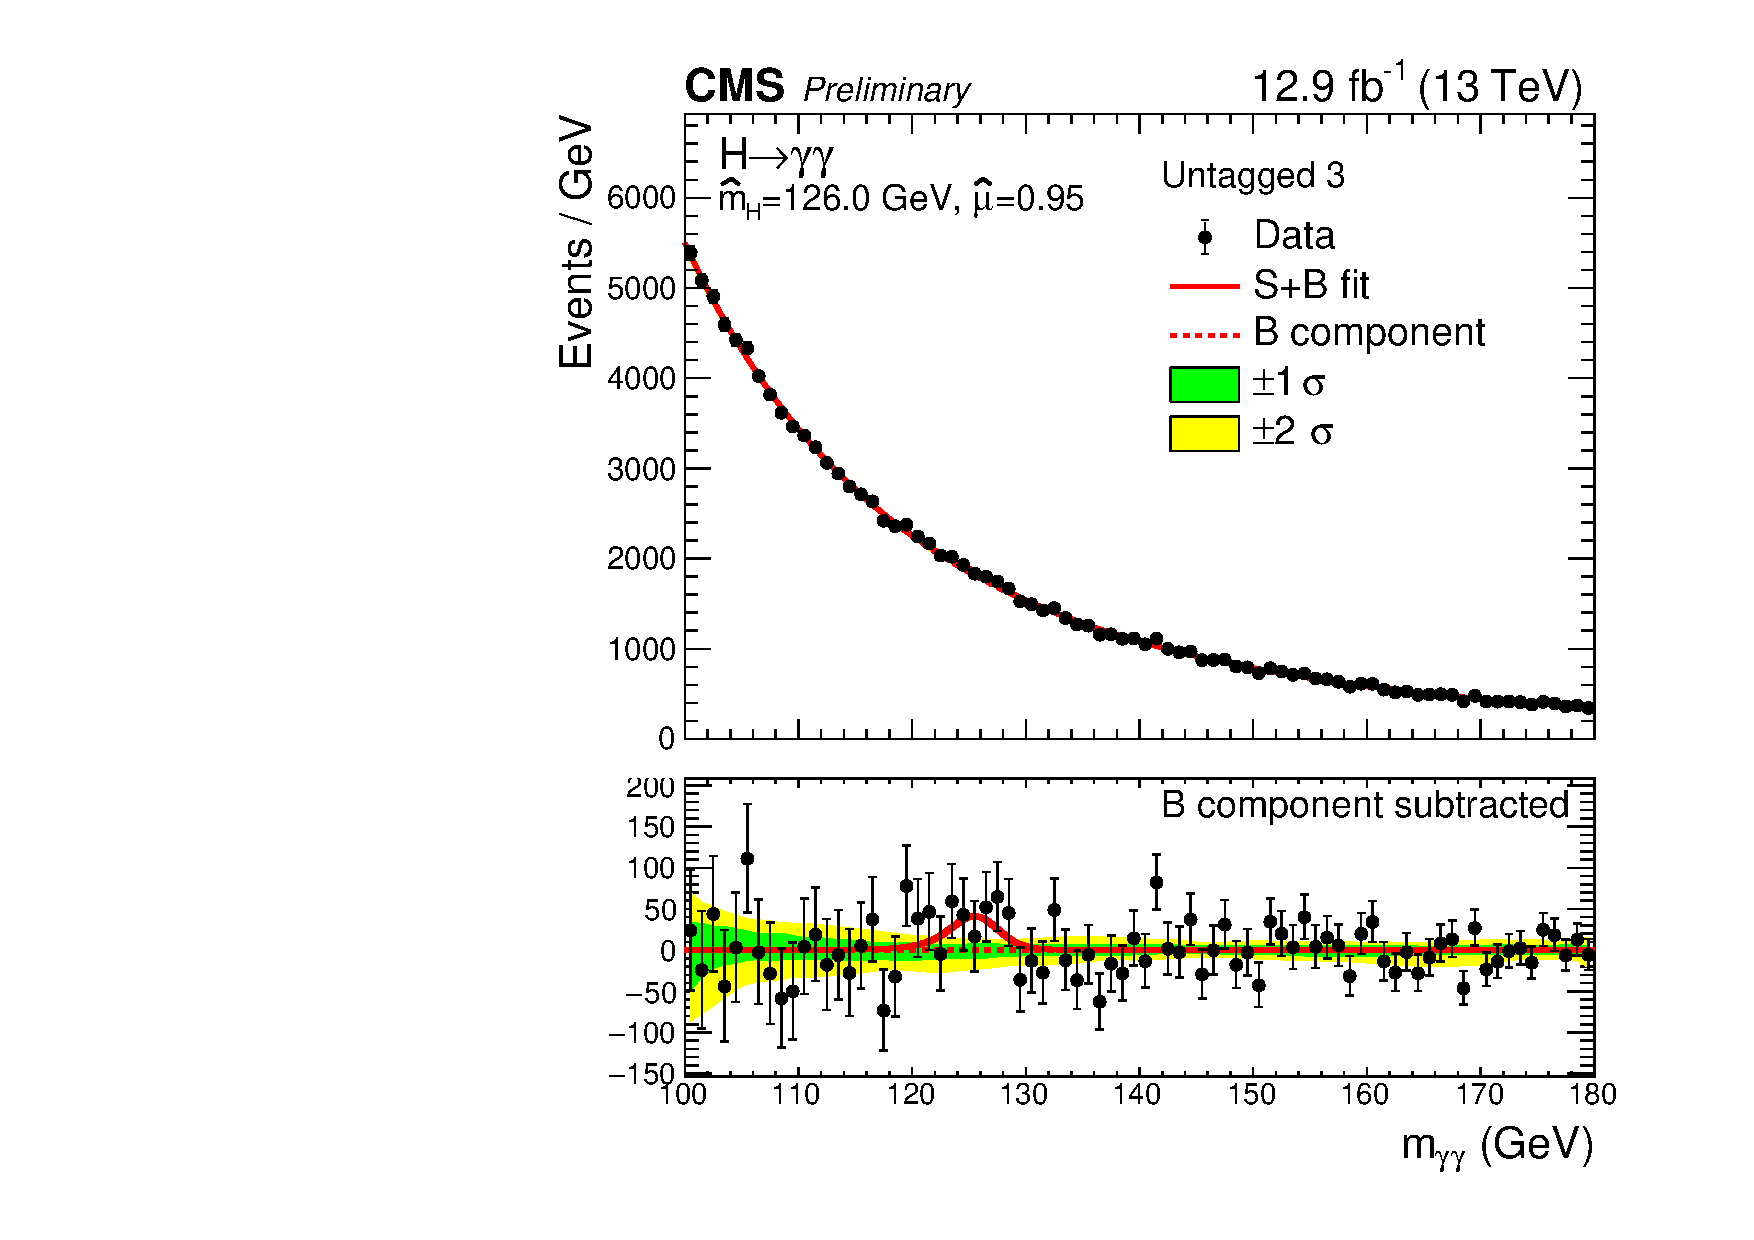
\includegraphics[width=0.49\textwidth]{statandresultsFigures/S_SB_ProfileMH_UntaggedTag_3_13TeV.pdf} \\
\caption{The signal-plus-background fit (solid red line) of the \mgg distribution in data (black points) for the \Untagged analysis categories. The background-only fit is shown as a dashed red line, while the green and yellow bands denote the $1\sigma$ and $2\sigma$ uncertainties on the background shape respectively.}

\label{fig:statandresults:s_b_fits}
\end{figure}

\begin{figure}[hpt!]
\centering
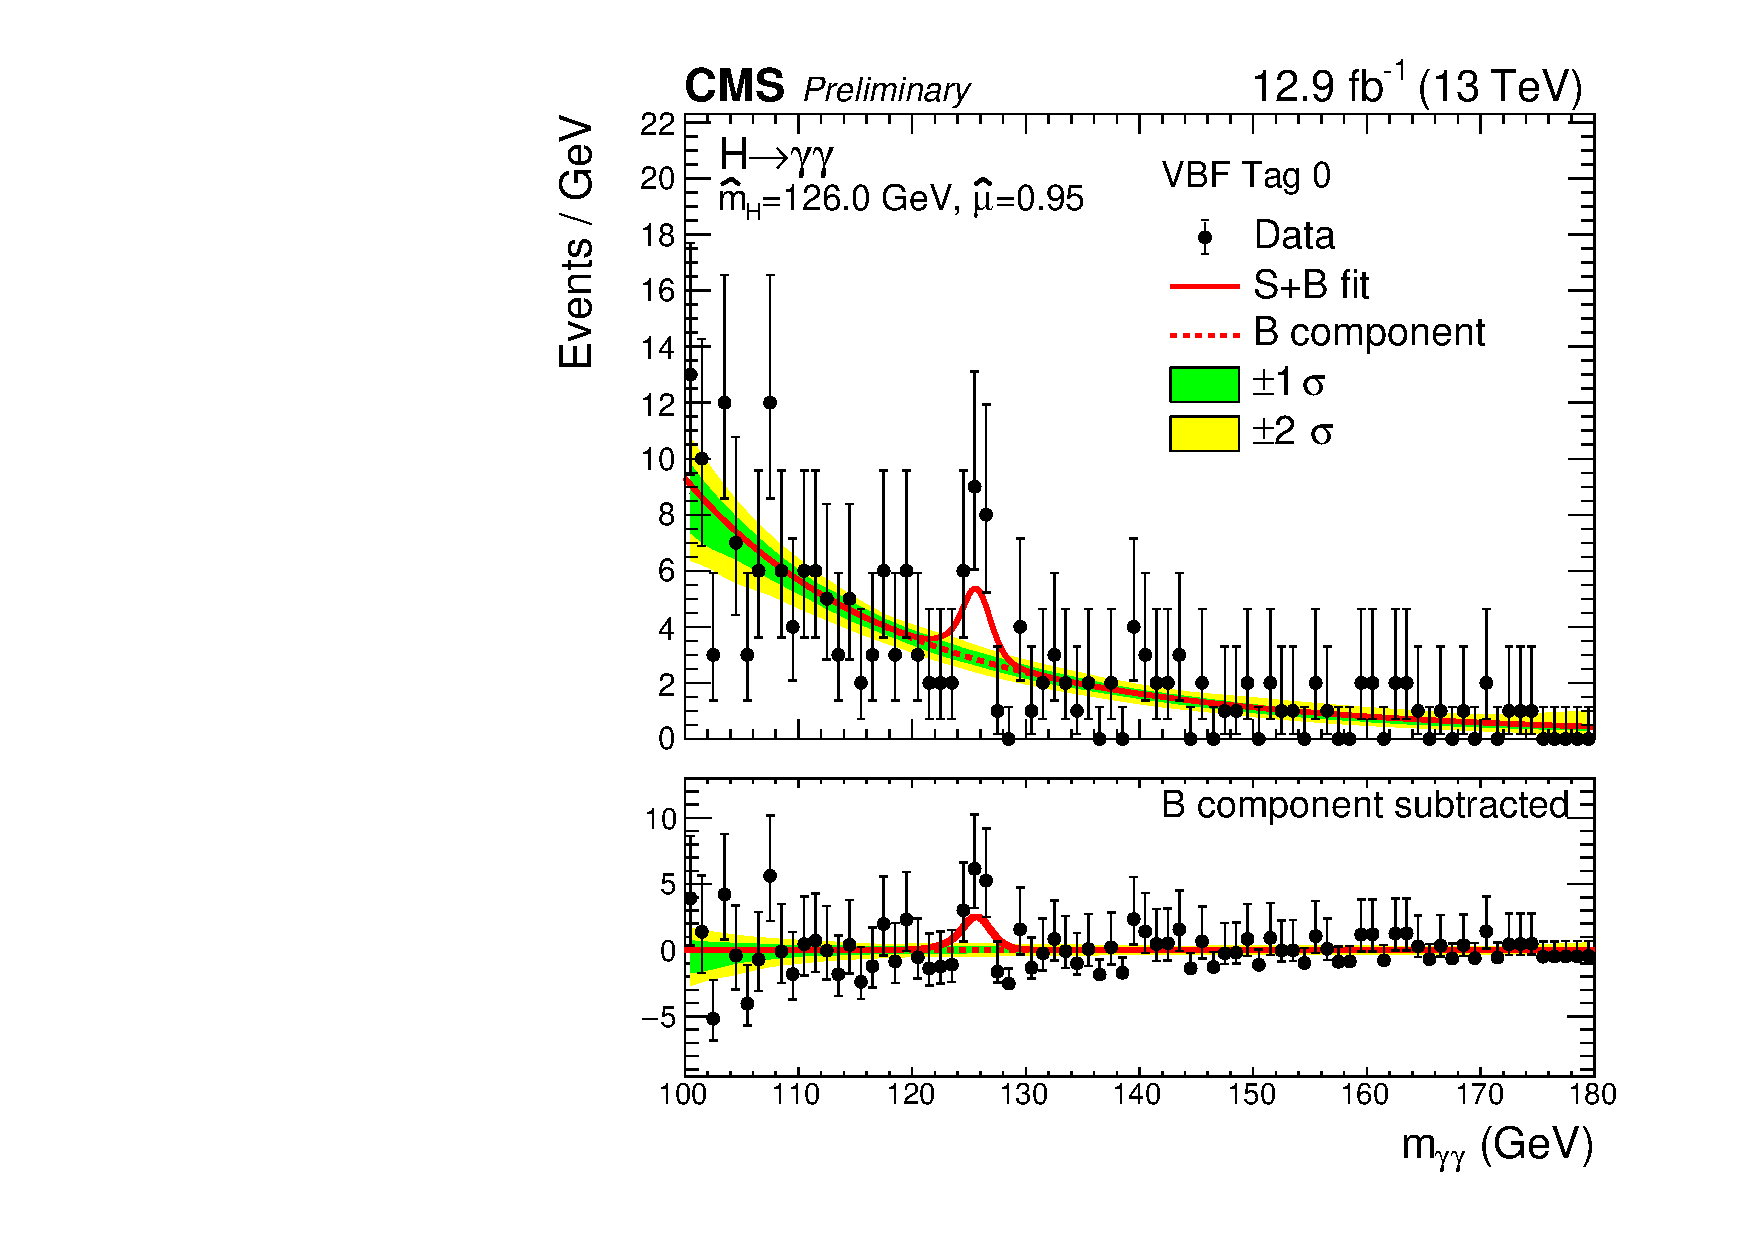
\includegraphics[width=0.49\textwidth]{statandresultsFigures/S_SB_ProfileMH_VBFTag_0_13TeV.pdf} 
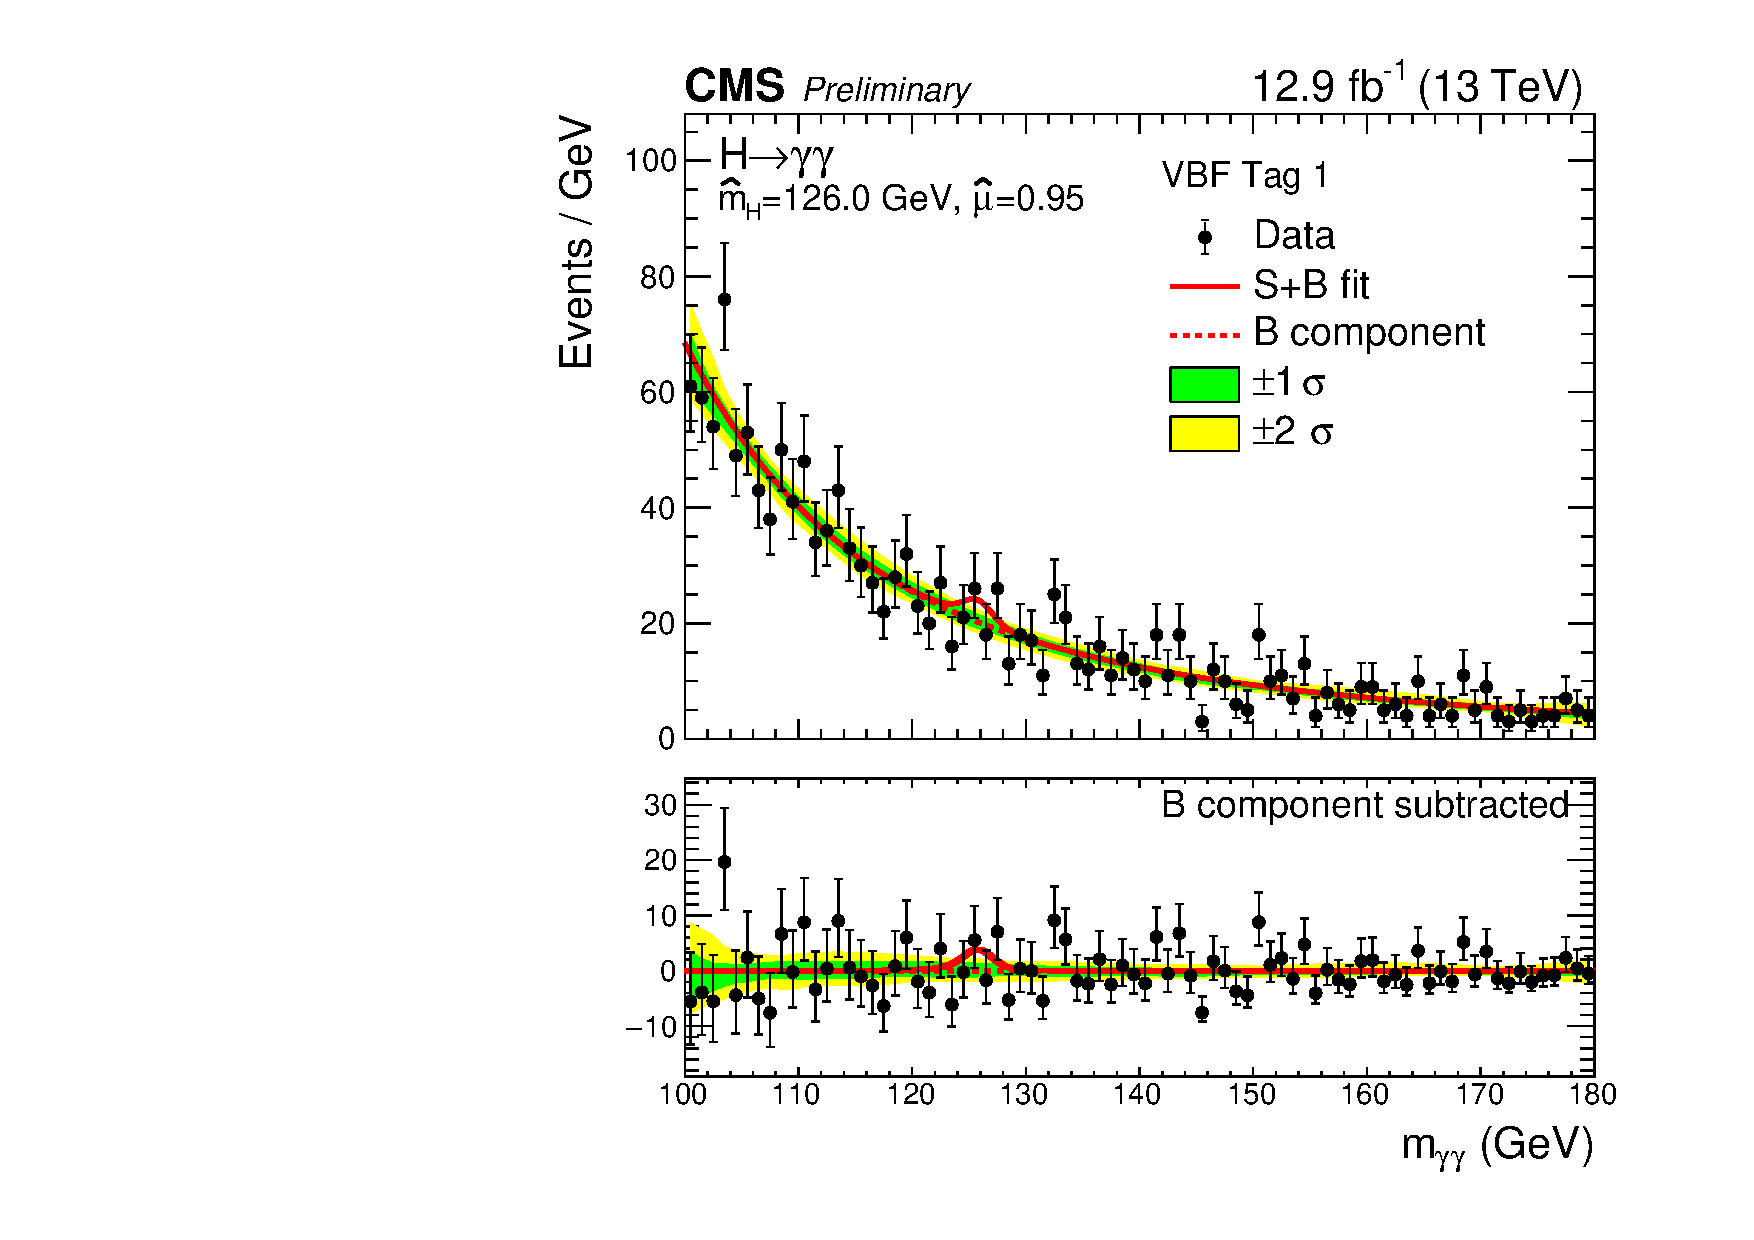
\includegraphics[width=0.49\textwidth]{statandresultsFigures/S_SB_ProfileMH_VBFTag_1_13TeV.pdf} 
%\includegraphics[width=0.3\textwidth]{statandresultsFigures/S_SB_ProfileMH_VBFTag_2_13TeV.pdf} 
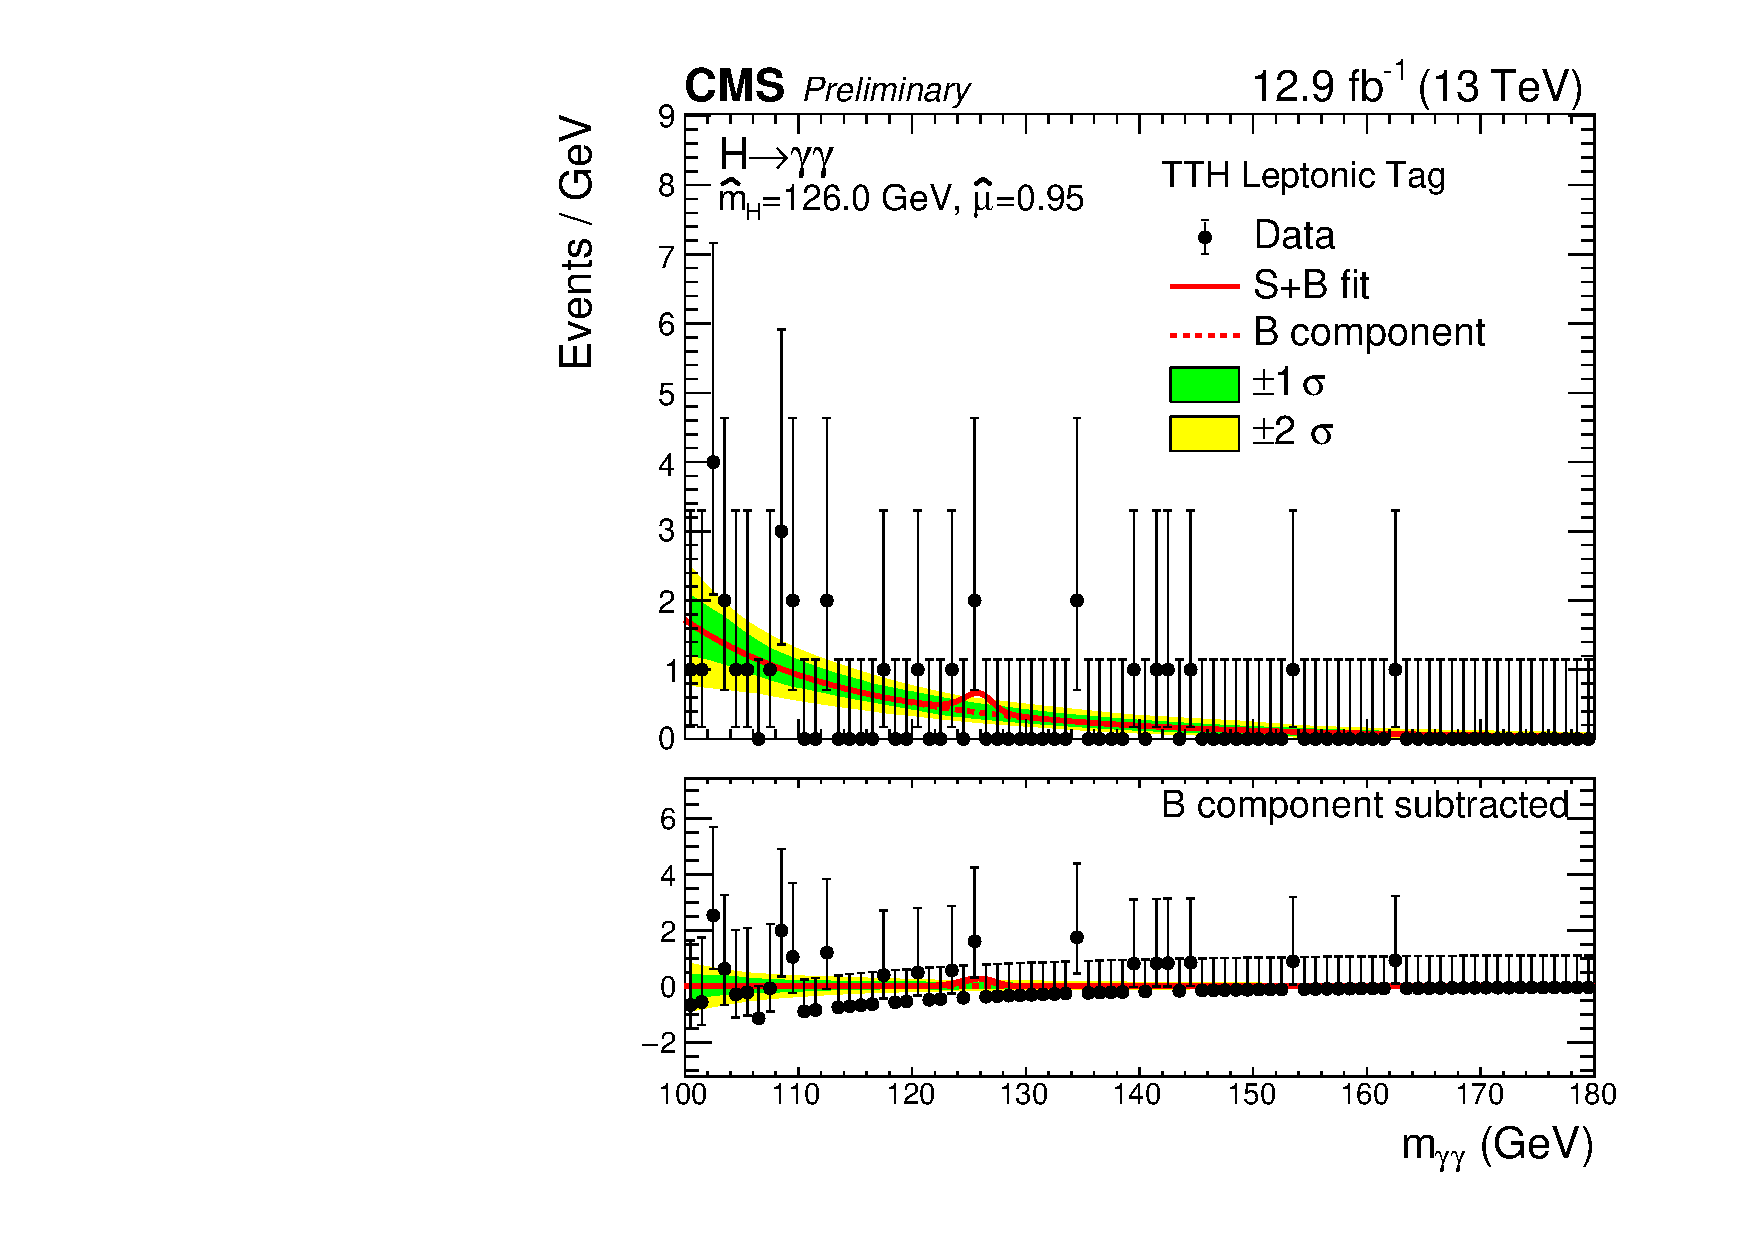
\includegraphics[width=0.49\textwidth]{statandresultsFigures/S_SB_ProfileMH_TTHLeptonicTag_13TeV.pdf} 
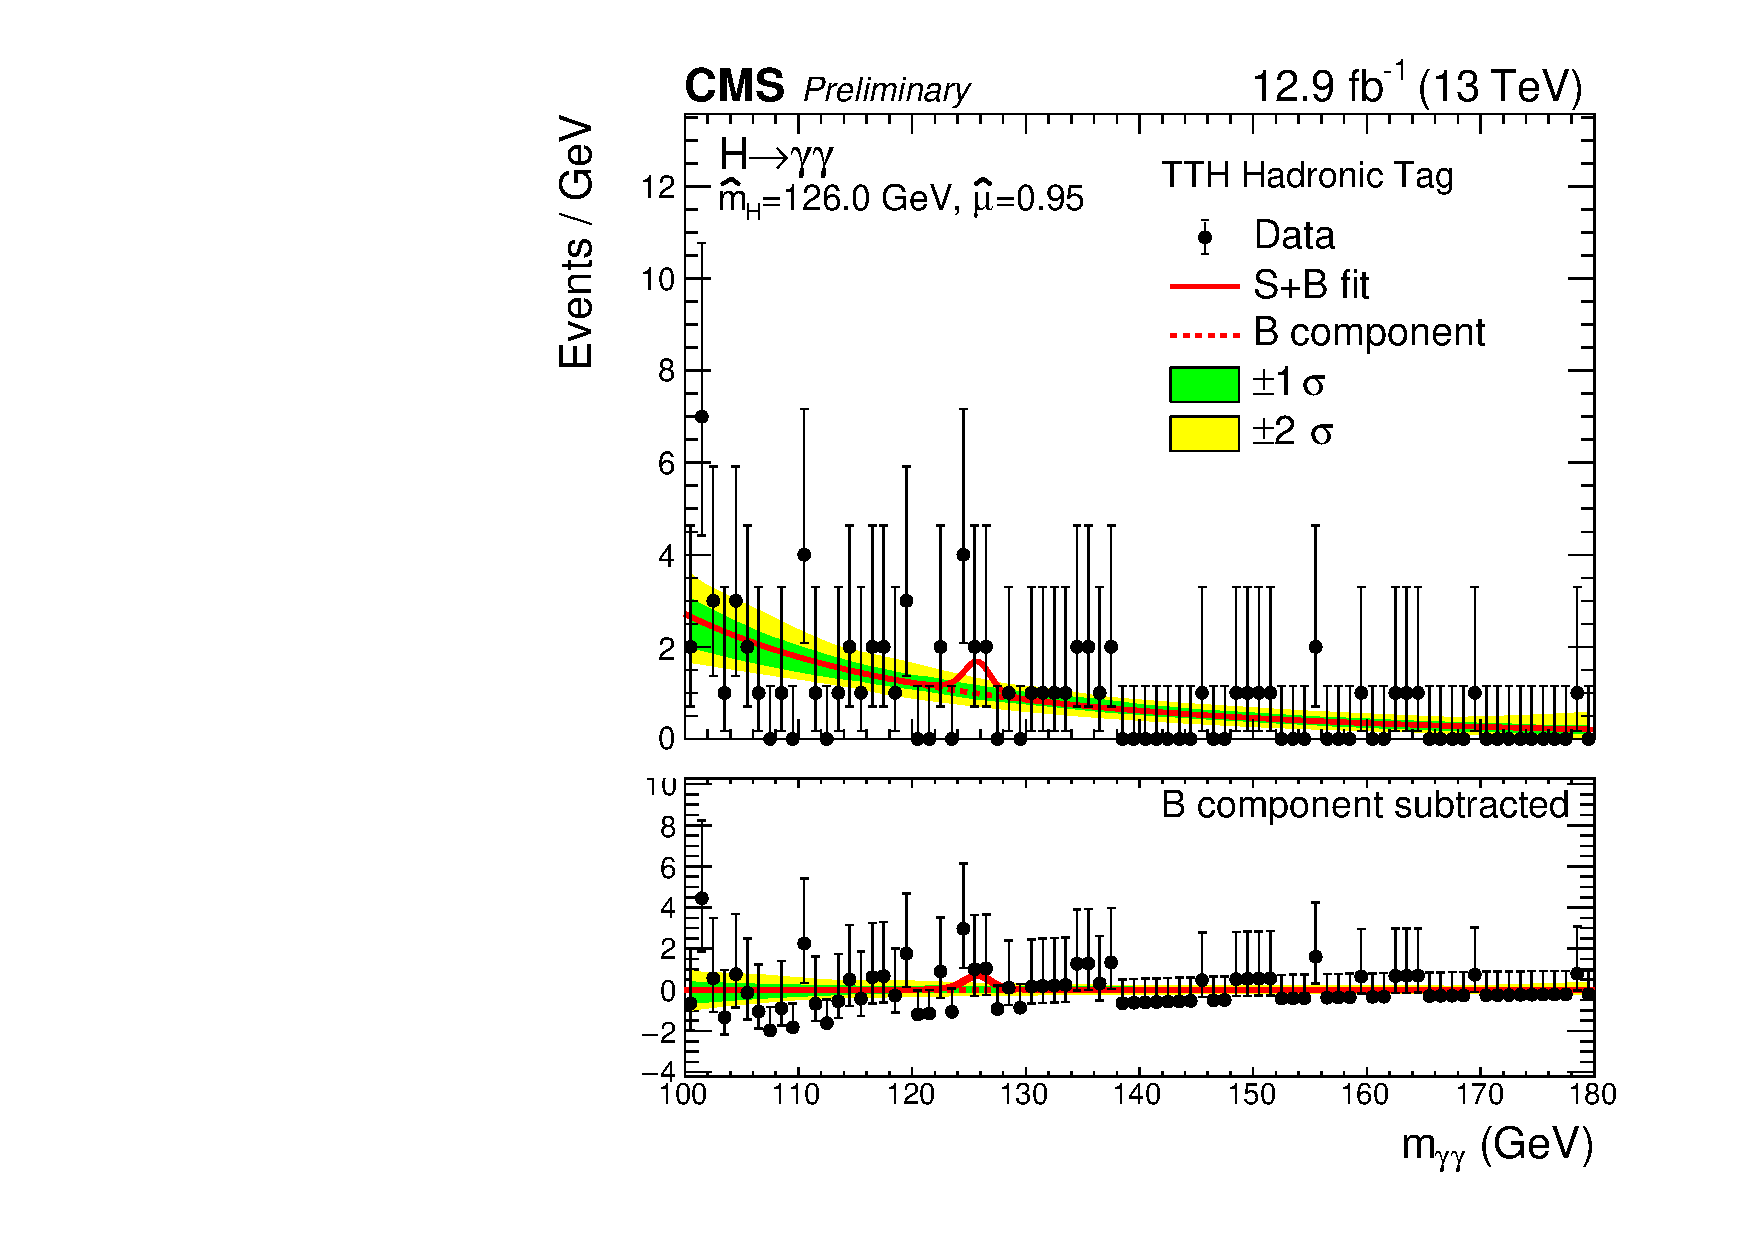
\includegraphics[width=0.49\textwidth]{statandresultsFigures/S_SB_ProfileMH_TTHHadronicTag_13TeV.pdf} \\
%\includegraphics[width=0.3\textwidth]{statandresultsFigures/S_SB_ProfileMH_VHLeptoniclooseTag_13TeV.pdf} 
%\includegraphics[width=0.3\textwidth]{statandresultsFigures/S_SB_ProfileMH_VHMetTag_13TeV.pdf} 
%\includegraphics[width=0.3\textwidth]{statandresultsFigures/S_SB_ProfileMH_VHHadronicTag_13TeV.pdf} \\
%\includegraphics[width=0.3\textwidth]{statandresultsFigures/S_SB_ProfileMH_WHLeptonicTag_13TeV.pdf} 
%\includegraphics[width=0.3\textwidth]{statandresultsFigures/S_SB_ProfileMH_ZHLeptonicTag_13TeV.pdf} 
\caption{The signal-plus-background fit (solid red line) of the \mgg distribution in data (black points) for the \VBFTag and \TTHTag analysis categories. The background-only fit is shown as a dashed red line, while the green and yellow bands denote the $1\sigma$ and $2\sigma$ uncertainties on the background shape respectively.}

\label{fig:statandresults:s_b_fits_bis}
\end{figure}

\begin{figure}[hpt!]
\centering
\subfloat[Direct sum]{
 \label{fig:statandresults:s_b_fits_direct_sum}
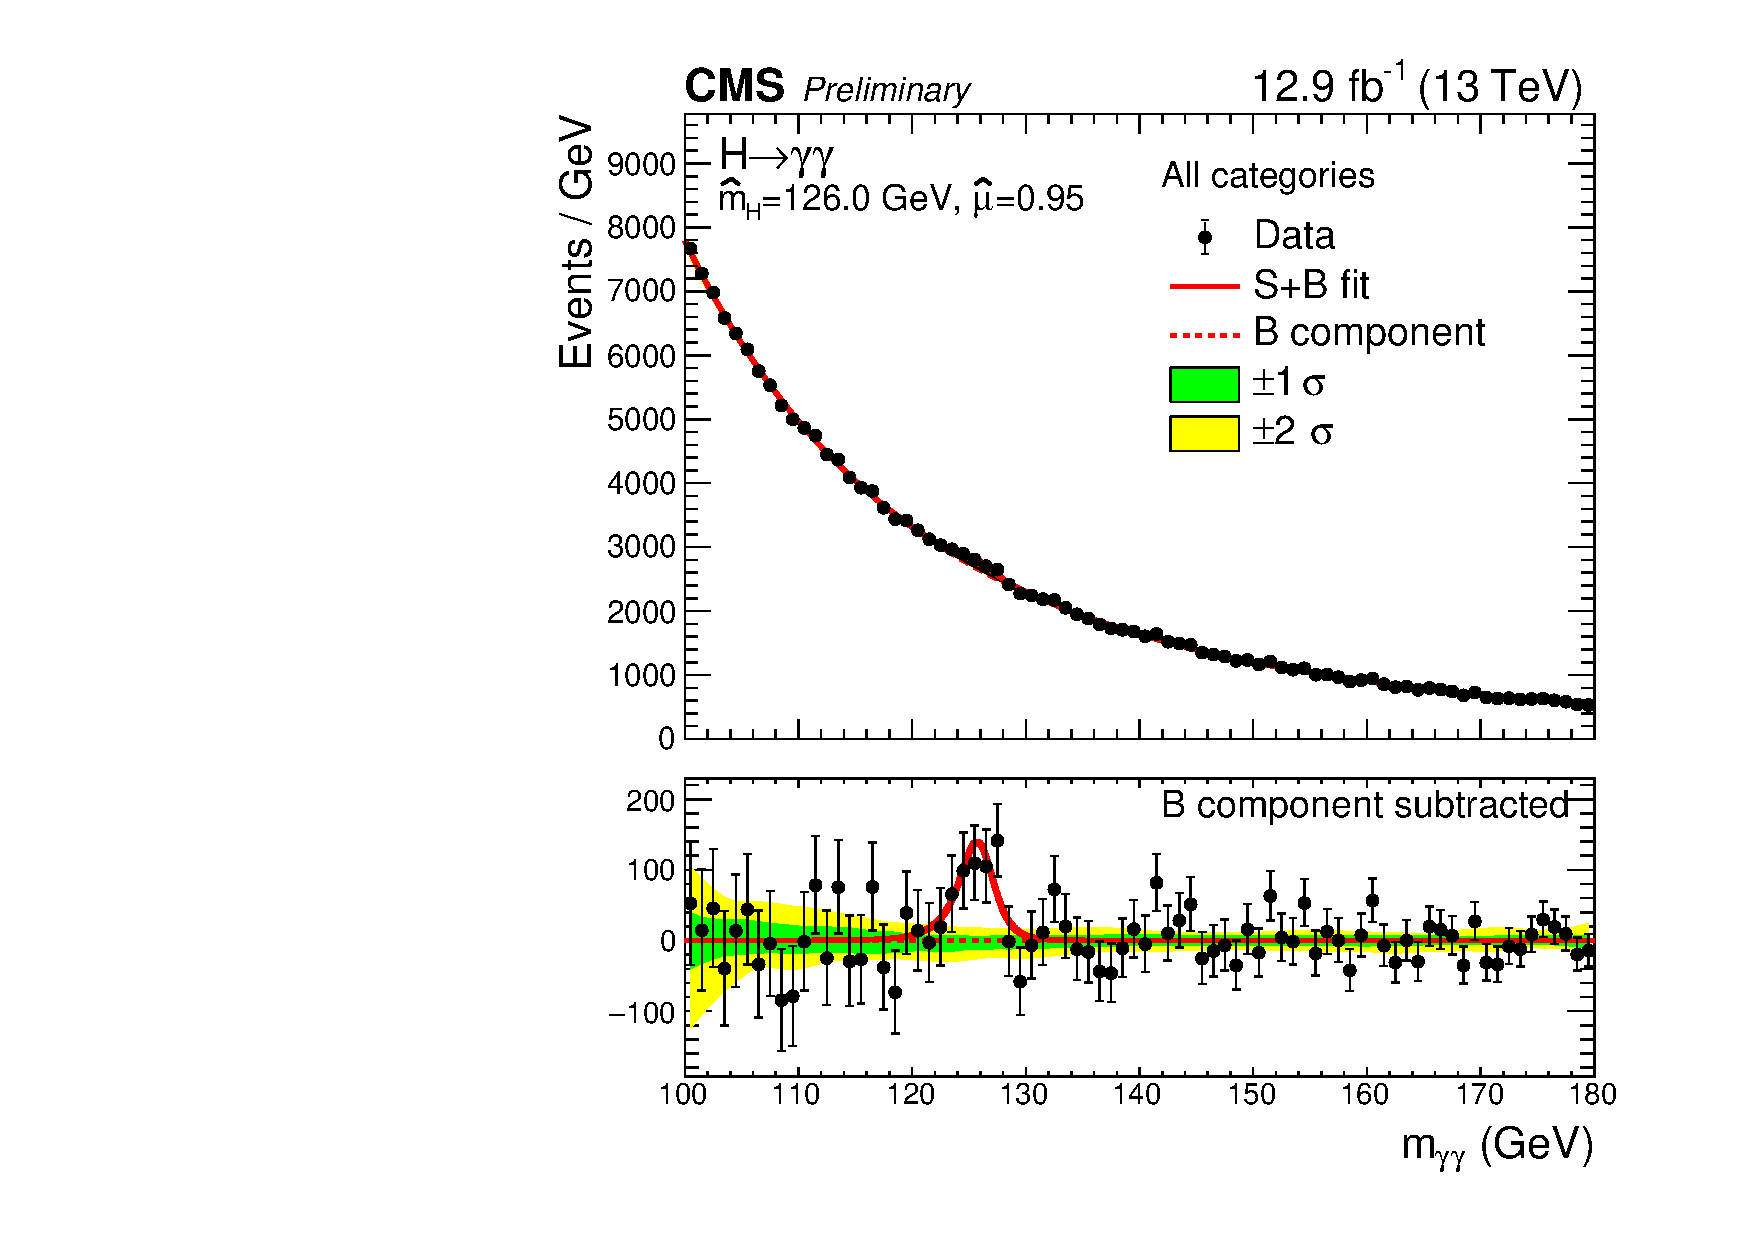
\includegraphics[width=0.59\textwidth]{statandresultsFigures/S_SB_ProfileMH_combcat_unweighted.pdf}}\\
\subfloat[S/(S+B) weighted sum]{
 \label{fig:statandresults:s_b_fits_s_sb_sum}
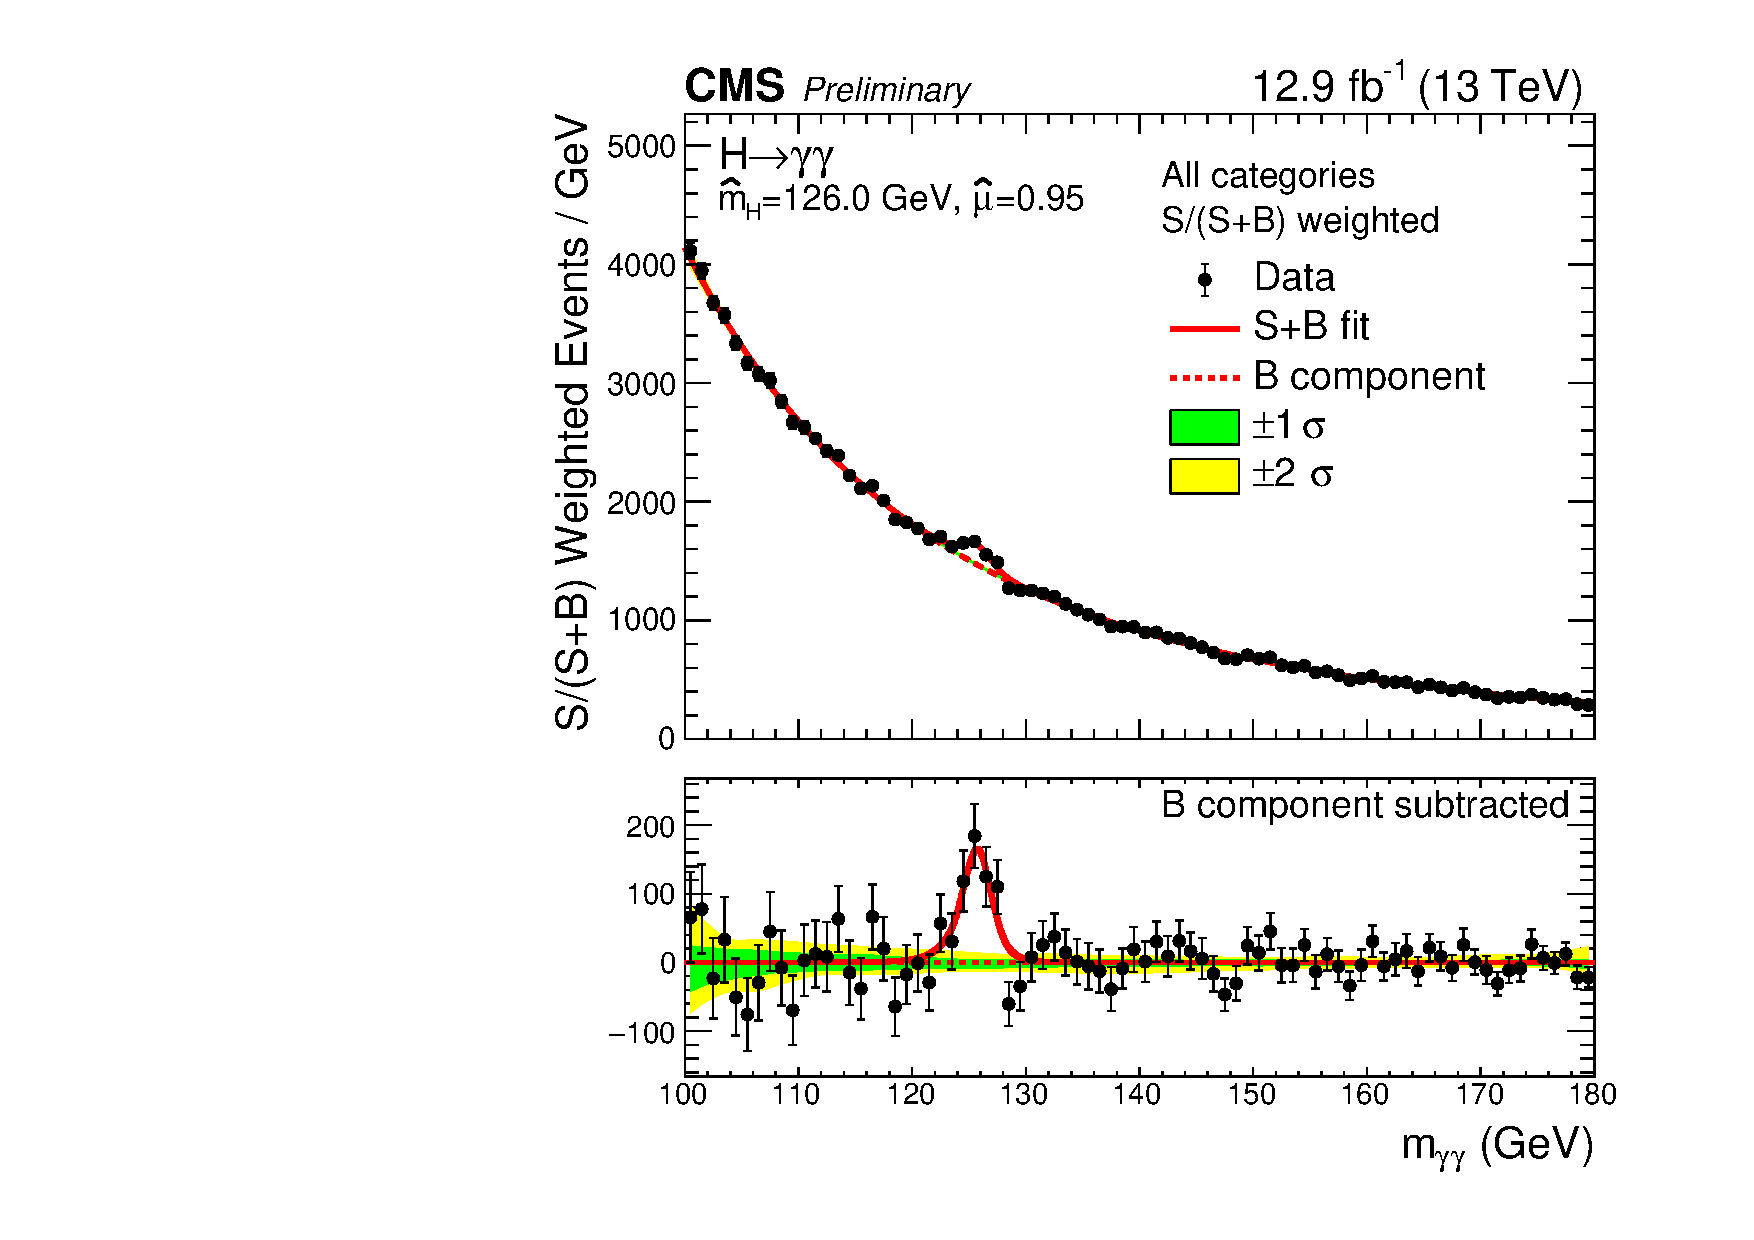
\includegraphics[width=0.59\textwidth]{statandresultsFigures/S_SB_ProfileMH_combcat_weighted.pdf}}
\caption{The signal-plus-background fit (solid red line) of the \mgg distribution in data (black points) for all categories combined, either using a direct sum (a) or a sum weighted by the $S/(S+B)$ in $\pm \effSigma$ around the best-fit value of \mH (b). The background-only fit is shown as a dashed red line, while the green and yellow bands denote the $1\sigma$ and $2\sigma$ uncertainties on the background shape respectively.}

\label{fig:statandresults:s_b_fits_sum}
\end{figure}


\section{Significance of observation}
\label{sec:statandresults:significance}

Given the best-fit value of the signal strength $\hat{\mu}= 0.95$ determined in \Sec~\ref{sec:statandresults:bestfit}, a frequentist approach is used to determine the degree of certainty with which the hypothesis that there is no Higgs boson can be rejected in favour of an alternative hypothesis which is that a \SM-like Higgs boson exists. The hypotheses can be formulated in terms of the signal strength: the null hypothesis $H_{0}$ corresponds to the case where $\mu=0$, while the alternative hypothesis $H_{\mu}$ corresponds to $\mu > 0$. 

A statistical test is constructed by specifying a critical region $w$ of the data space, such that for a given set of observed data $\mgg^{obs}$:
\begin{equation}
P(\mgg^{obs} \in w | H_{0} ) \leq \alpha,
\end{equation}

where  $P(\mgg^{obs} \in w | H_{0} ) $ is the probability (assuming that $H_{0}$ is correct), of observing the data inside the critical region $w$, and $\alpha$ is a small predetermined threshold~\cite{Cowan}. 

The statistical power $\beta$ of the test is the probability of accepting $H_{0}$ when it is false and the alternative $H_{\mu} $ is true. This is given by:

\begin{equation}
P(\mgg^{obs} \in  w | H_{\mu} ) = 1 - \beta.
\end{equation}

The critical region should be chosen such that the power $\beta$ of the test is maximised for a given $\alpha$, to ensure that if $\mgg^{obs} \in w$, then $H_{0}$ has a low probability of being true while $H_{\mu}$ has a high probability of being true.  

A common choice, which is found to maximise $\beta$~\cite{Cowan}, is to define the critical region in terms of a test statistic $q_{\mu}$, corresponding to the difference between the best-fit \NLL and the \NLL evaluated for a particular $\mu$. This difference is abbreviated as \DNLL, and can be expressed as:
\begin{equation}
q_{\mu} = \begin{cases} 
  -2 \ln \mathcal{L}(\mu,\hat{\mH}^{\mu} ; \hat{\mathbf{n}}^{\mu}| \mgg^{obs})- \ln\mathcal{L}(\hat{\mu},\hat{\mH} ;\hat{\mathbf{n}}| \mgg^{obs} ) & \text{when } \hat{\mu} \geq 0, \\
  0 & \text{when } \hat{\mu} < 0, 
  \end{cases}
\end{equation}

where $\hat{\mH}^{\mu}$ and $\hat{\mathbf{n}}^{\mu}$ denote the best-fit values $\mH$ and $\mathbf{n}$ for a fixed value of $\mu$. In this case, \mH is said to be \emph{profiled}, although the test statistic can be modified to evaluate the \DNLL for a given \mH hypothesis by fixing it to a particular value instead. 
When trying to exclude hypothesis $H_{0}$, the test statistic $q_{0}$ in particular should be used to define a critical region. In the limit of a large sample of data, the probability distribution function of the test statistic ($f_q$), is Gaussian. The fact that $q_{0} =0$ for $\hat{\mu} < 0$ reflects the fact that only excesses in the data are regarded as significant. This simplifies the definition of the critical region, since increasingly large values of $q_{0}$ indicate increasing incompatibility with $H_{0}$, and therefore only the right-hand tail of $f_q$ is considered when assessing probabilities. Assuming $H_{0}$, the probability of obtaining a value of $q^{{obs}}_{0}$ (corresponding to observed data $ \mgg^{obs}$) or higher is given by the integral of $f_q$ from $q^{{obs}}_{0}$ to infinity. This probability is commonly referred to as the \pvalue. We can therefore define the critical region as:  

\begin{equation}
w = \{ \mgg^{obs} : \int_{q^{{obs}}_{0}}^{+\infty} f_q(q_{0}) dq_0  \leq \alpha \},
\end{equation}

In particle physics experiments, the threshold $\alpha$ to reject the null hypothesis is typically $2.87 \times 10^{-7}$. If expressed as the number of standard deviations that a Gaussian-distributed variable would fluctuate to give the same \pvalue, then this threshold is $5\sigma$.

The \pvalue can be evaluated separately for different assumption about the value of \mH. In this case, the value of \mH is fixed to the given value rather than being profiled in the \DNLL minimisation. The result of a scan of the \pvalue\s as a function of \mH in 0.1\GeV steps is shown in \Fig~\ref{fig:statandresults:pval}. The black solid line represents the \pvalue scan for the observed data. The dashed lines represent the expected \pvalue\s for a \SM Higgs boson. These are obtained by generating an Asimov dataset~\cite{Cowan:2010js} from the best-fit background-only model and a signal of strength $\mu=1$, and then performing a signal-plus-background fit as for oberved data. For the blue dashed line, the signal was injected at $\mH=125.09\GeV$ (the best fit value from the previous combined measurement of the Higgs boson mass by \CMS and \ATLAS~\cite{PhysRevLett.114.191803}), while for the red dashed line the signal was injected at the corresponding \mH for each step. 

The observed significance at $\mH=125.09\GeV$ is $5.6\sigma$, where $6.2\sigma$ was expected for the \SM Higgs boson. The maximum observed significance is found at $\mH=126.0\GeV$, corresponding to $6.1\sigma$.
Since the observed data fall in the critical region where the signifiance is above $5\sigma$ (i.e \pvalue is less than $2.87 \times 10^{-7}$), the null hypothesis that there is no Higgs boson is rejected. Therefore, the data correspond to a new observation of the Higgs boson decaying to photons.

\begin{figure}[ht!]
\centering
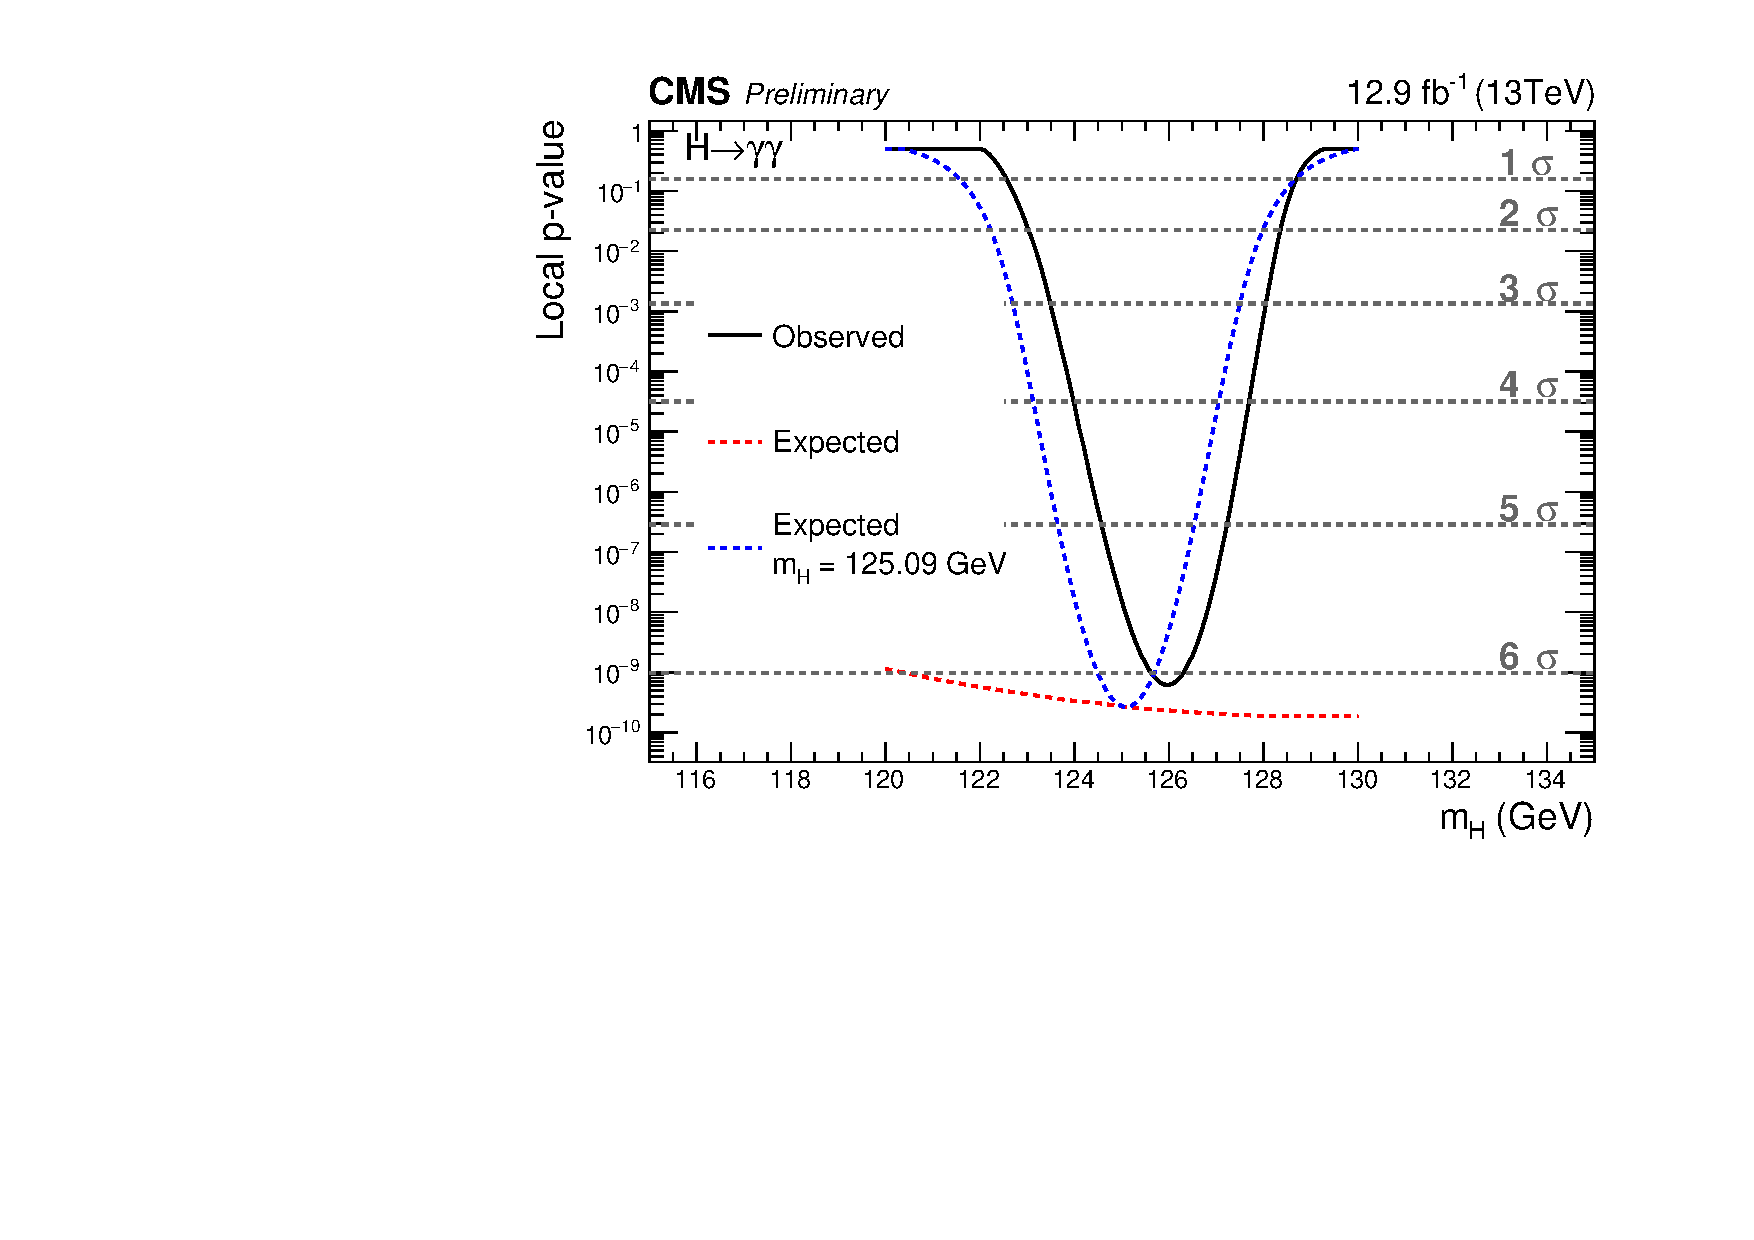
\includegraphics[width=0.9\textwidth]{statandresultsFigures/pval13TeV-observed.pdf} 
\caption{The \pvalue for the observation as a function of the Higgs boson mass (black), shown with the expected \pvalue\s for a SM Higgs boson, across the range 120-130\GeV. The expected \pvalue\s are obtained using Asimov datasets~\cite{Cowan:2010js}. The blue dashed line shows the expected \pvalue when the mass of the injected signal is $\mH=125.09\GeV$, while the red line shows the maximum significance for any injected signal in the range of $120$ to $130\GeV$.}

\label{fig:statandresults:pval}
\end{figure}

\section{Measurements of the signal strength}
\label{sec:statandresults:sigstrength}
\subsection{Global signal strength}
\label{sec:statandresults:sigstrength_global}

One of the advantages of using \DNLL as a test statistic is that to a very good approximation, the $\pm 1 \sigma$ uncertainty on the measured value of the \POI can be obtained by finding the values for which $\DNLL=1$~\cite{Cowan}. %$q_{\mu}=q_{\hat{\mu}}+1$~\cite{Cowan}.
This fact is used to produce a measurement of the global signal strength $\mu$. 

\Fig~\ref{fig:statandresults:global_mu} shows the value of \DNLL evaluated for fixed values of $\mu$ in small steps in the range of $0.5$ to $1.5$. This type of plot is referred to as a \DNLL \emph{scan}. In this case, \mH is profiled in the minimisation at each step. By definition, the best-fit point $\hat{\mu}$ has a \DNLL value of $0$. This gives the central value for the measurement. The upper and lower uncertainties are obtained by graphically finding the intercepts of the curve with \DNLL$=1$. 
The contribution to the total uncertainty on the signal strength arising from the statistical, theory systematic and experimental systematic components are assessed by freezing the corresponding nuisance parameters, and calculating the difference in quadrature with respect to the total uncertainty. 
The measured value of the signal strength is:
\begin{equation*}
\hat{\mu}=0.95 ^{+0.21}_{-0.19} = 0.95 \pm 0.17 \text{ (stat.) }^{+0.09}_{-0.06} \text{ (theo. syst.) }^{+0.10}_{-0.07} \text{ (exp. syst.)}. 
\end{equation*}
This measurement indicates that the observed global signal strength is compatible with the \SM expectation within one standard deviation.

\begin{figure}[ht!]
\centering
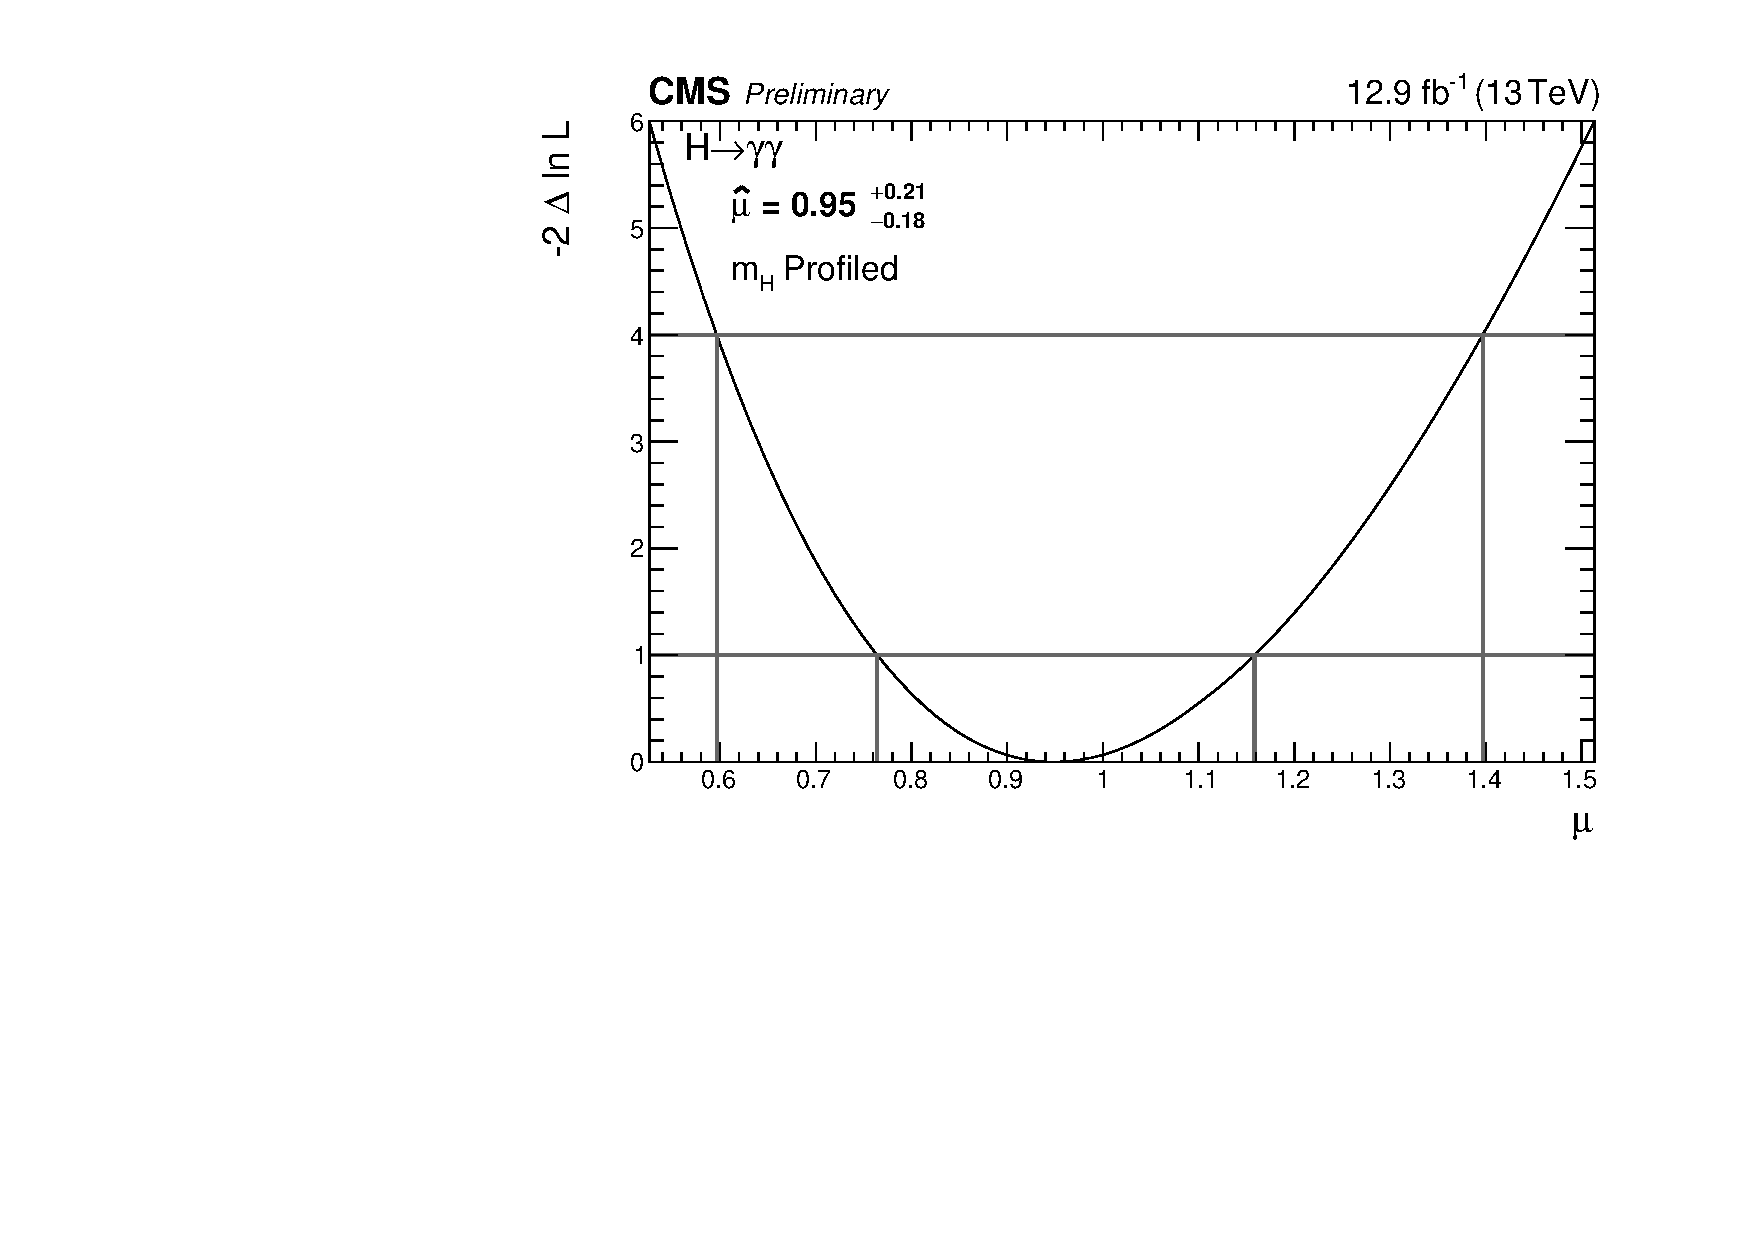
\includegraphics[width=0.9\textwidth]{statandresultsFigures/MuScanProfileMH.pdf} 
\caption{The \DNLL scan of the overall signal strength for a Higgs boson decaying to two photons. The mass of the Higgs boson is profiled in the fit. The $1\sigma$ and $2\sigma$ uncertainties correspond to the crossings with \DNLL$=1$ and \DNLL=$4$.}

\label{fig:statandresults:global_mu}
\end{figure}

Instead of allowing the \mH parameter the be profiled, it can instead be fixed to particular values. A similar likelihood scan can be repeated for given values of \mH in the 120-130\GeV range, in small steps. The result is shown in \Fig~\ref{fig:statandresults:mu_vs_mh}, where the best-fit signal strength is plotted as a function of the fixed value of \mH, where the green bands represent the $\pm 1 \sigma$ uncertainty obtained by finding the crossing with \DNLL$=1$ as described above. This figure illustrates that no other excesses other than the one at the best-fit exist in the region of interest.  

\begin{figure}[ht!]
\centering
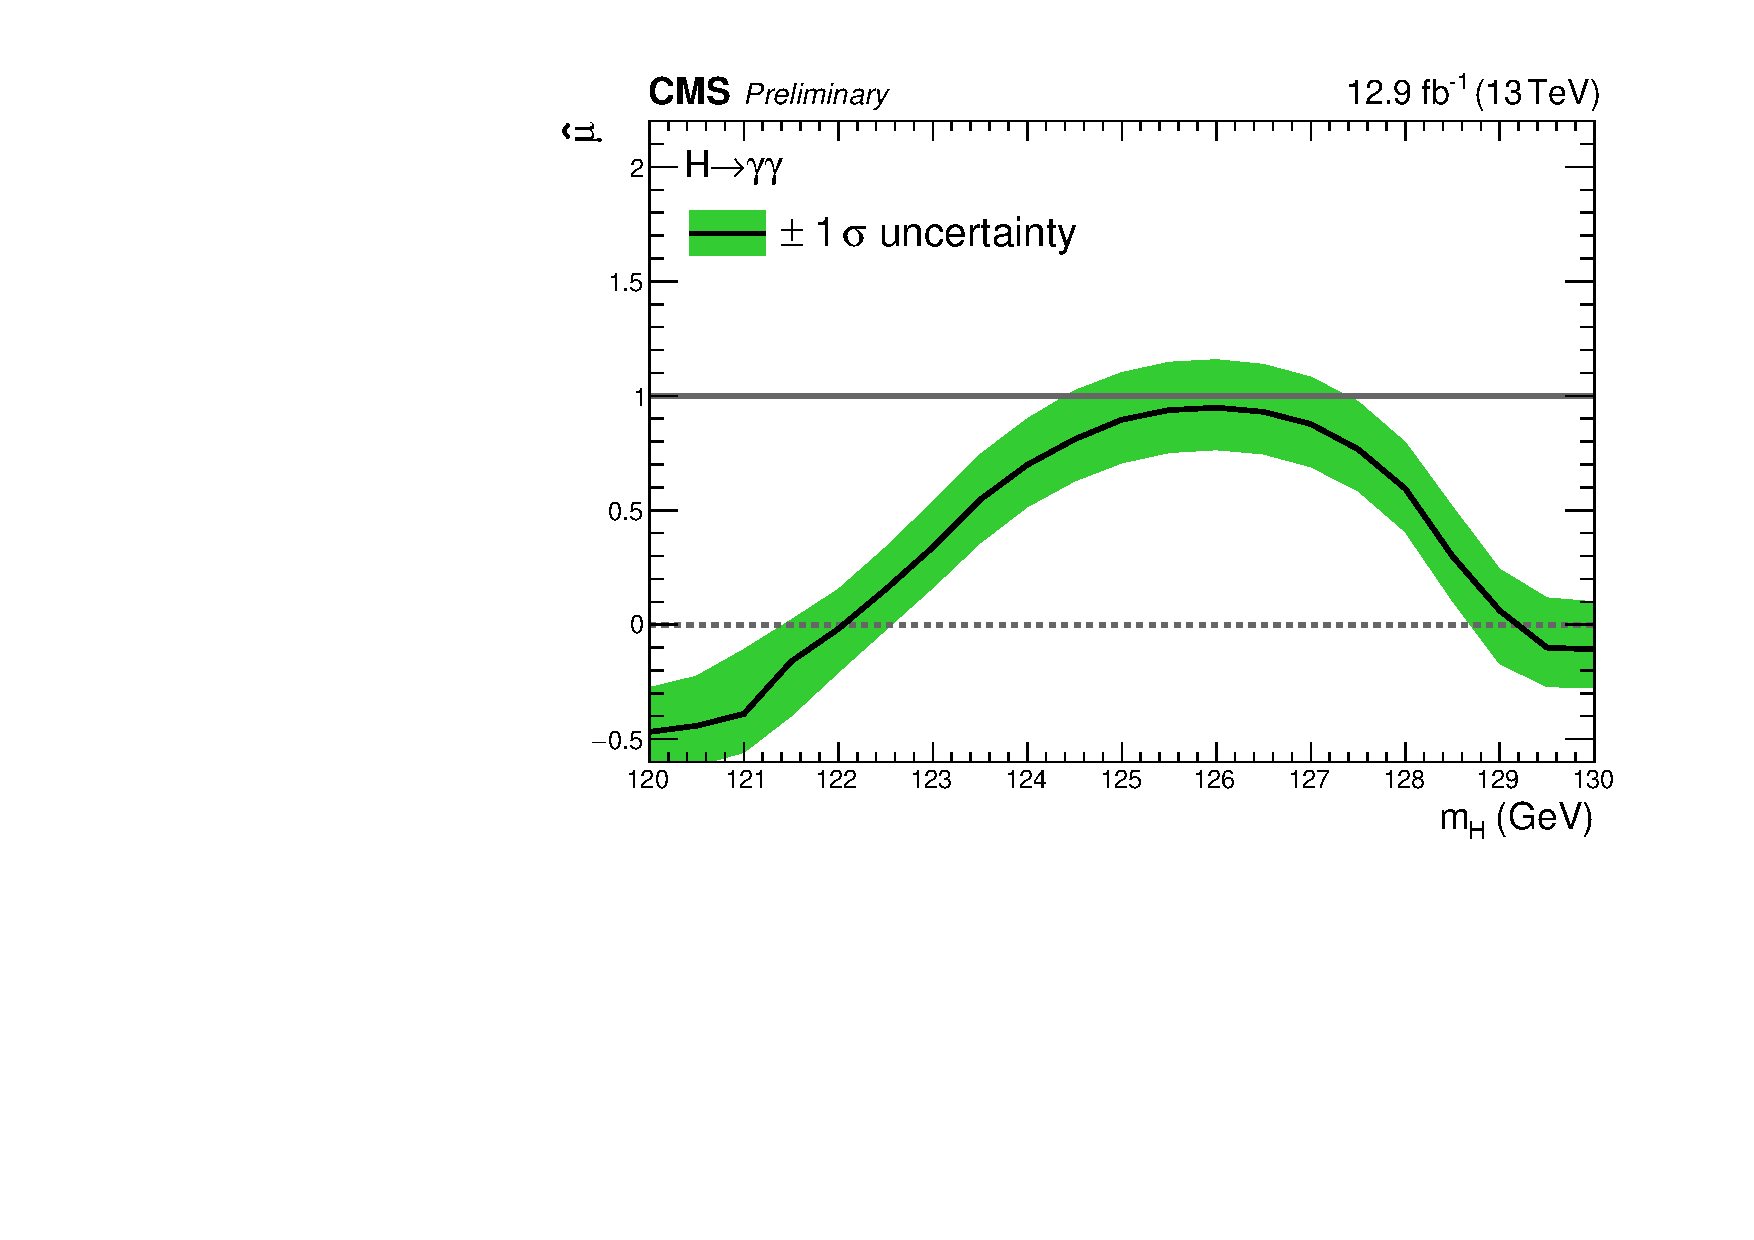
\includegraphics[width=0.9\textwidth]{statandresultsFigures/MuHat_vs_MH.pdf} 
\caption{The best-fit signal strength for fixed values of \mH in the 120-1230\GeV range, where the \mH parameter is fixed in the fitting procedure. The green bands show  the $\pm 1 \sigma$ uncertainty obtained by finding the crossing with \DNLL$=1$.  }

\label{fig:statandresults:mu_vs_mh}
\end{figure}

\subsection{Fermionic and bosonic components of the signal strength}
\label{sec:statandresults:rvrf}

When making the measurement of the global signal strength as in \Sec~\ref{sec:statandresults:sigstrength_global}, a single \POI which uniformly scales all production processes in all categories is defined. However, this measurement makes the assumption that the contribution of each production process to the total Higgs boson \crosssection is in proportion to the \SM prediction. In order to test this assumption, the single \POI representing to global signal strength can be split up into components. For example, the contributions from the production modes where the Higgs boson is produced from fermions (\ggH and \ttH) and vector bosons (\VBF and \VH) are separated, to test if they individually agree with the \SM expectation.

The measurement is made by producing a two-dimensional \DNLL scan with a slightly modified test statistic, where two \POI\s, \muF and \muV, are considered in the place of $\mu$. The likelihood function is modified such that the \muF parameter scales the yield of the signal models for the \ggH and \ttH processes in all categories uniformly, but does not affect the yields of the models for the \VBF or \VH processes, and vice-versa for the \muV parameter. The \mH parameter is profiled in the scan.

The result of the two-dimensional scan can be seen in \Fig~\ref{fig:statandresults:mu_per_rvrf}. The $z$-axis, representing the value of \DNLL, has been omitted for clarity.  The black cross shows the location of the best-fit point, with the red diamond indicating the \SM expectation. The $1\sigma$ and $2\sigma$ contours, which represent the intersection with $\DNLL=2.30$ and $\DNLL=6.18$ respectively, are shown as solid and dashed lines. The plot shows that the observed best-fit of $(\muF ,\muV )=(0.82,1.60)$ is consistent with the \SM hypothesis within $1\sigma$.
\begin{figure}[ht!]
\centering
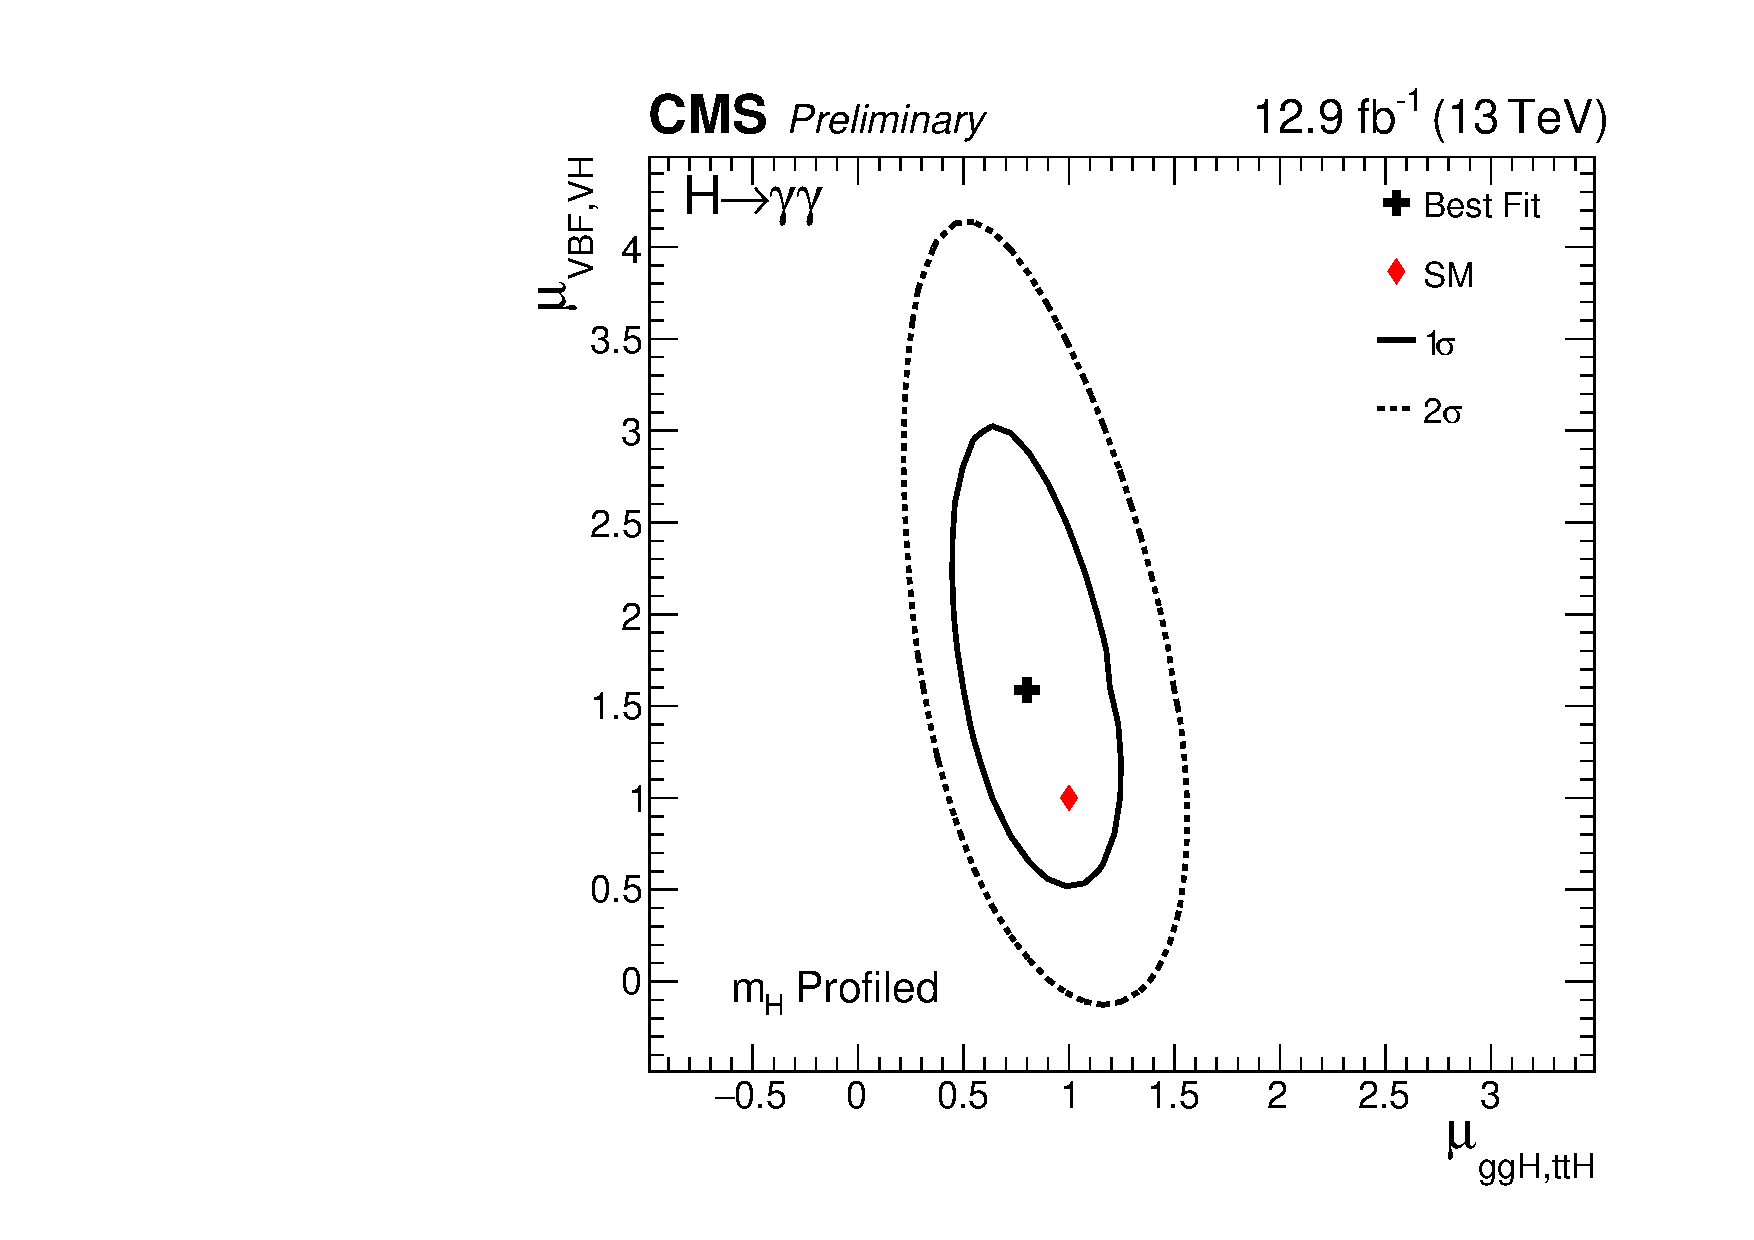
\includegraphics[width=0.8\textwidth]{statandresultsFigures/RVRFScanProfileMH.pdf} 
\caption{The result of a two-dimensional \DNLL scan of the \muF and \muV components of the signal strength. The red diamond indicates the SM expectation, while the black cross shows the location of the best-fit point. The measurement is consistent with the SM within the uncertainty contours, which are shown in dashed lines. The value of \mH was profiled in the scan.}

\label{fig:statandresults:mu_per_rvrf}
\end{figure}

To correctly extract the uncertainties on \muF and \muV individually, a \DNLL scan of each parameter is performed while profiling the other. The resulting scans can be seen in \Fig\s~\ref{fig:statandresults:mu_per_rv} and~\ref{fig:statandresults:mu_per_rf}. The result of the measurement is found to be:
\begin{equation*}
\muFhat=0.82^{+0.27}_{-0.24} \text{ and } \muVhat=1.60^{+0.90}_{-0.76}. 
\end{equation*}
The fermionic and bosonic components of the signal strength are therefore found to be compatible with the \SM expectations. 

\begin{figure}[ht!]
\centering
\subfloat[\DNLL scan of \muV, profiling \muF and \mH]{
\label{fig:statandresults:mu_per_rv}
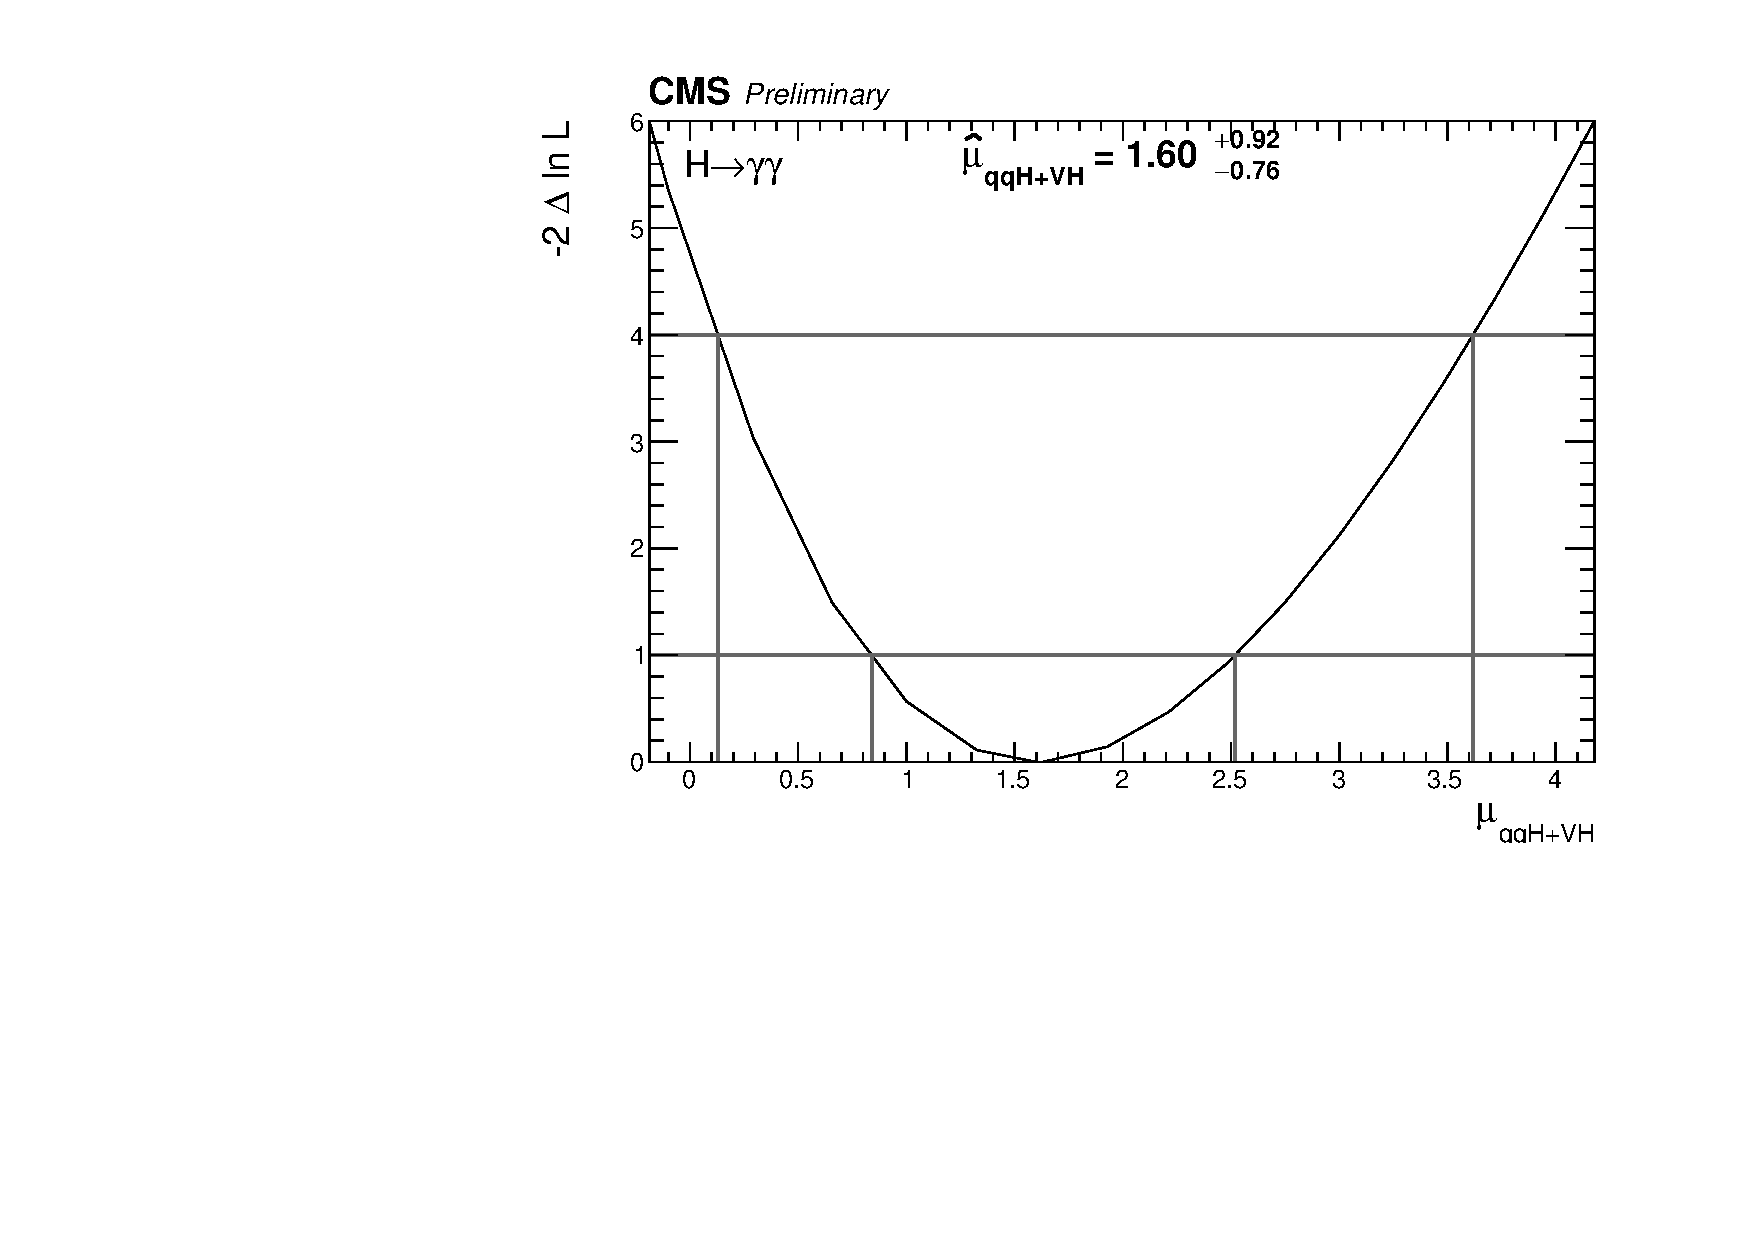
\includegraphics[width=0.83\textwidth]{statandresultsFigures/RVScanProfileMH.pdf}} \\
\subfloat[\DNLL scan of \muF, profiling \muV and \mH]{
\label{fig:statandresults:mu_per_rf}
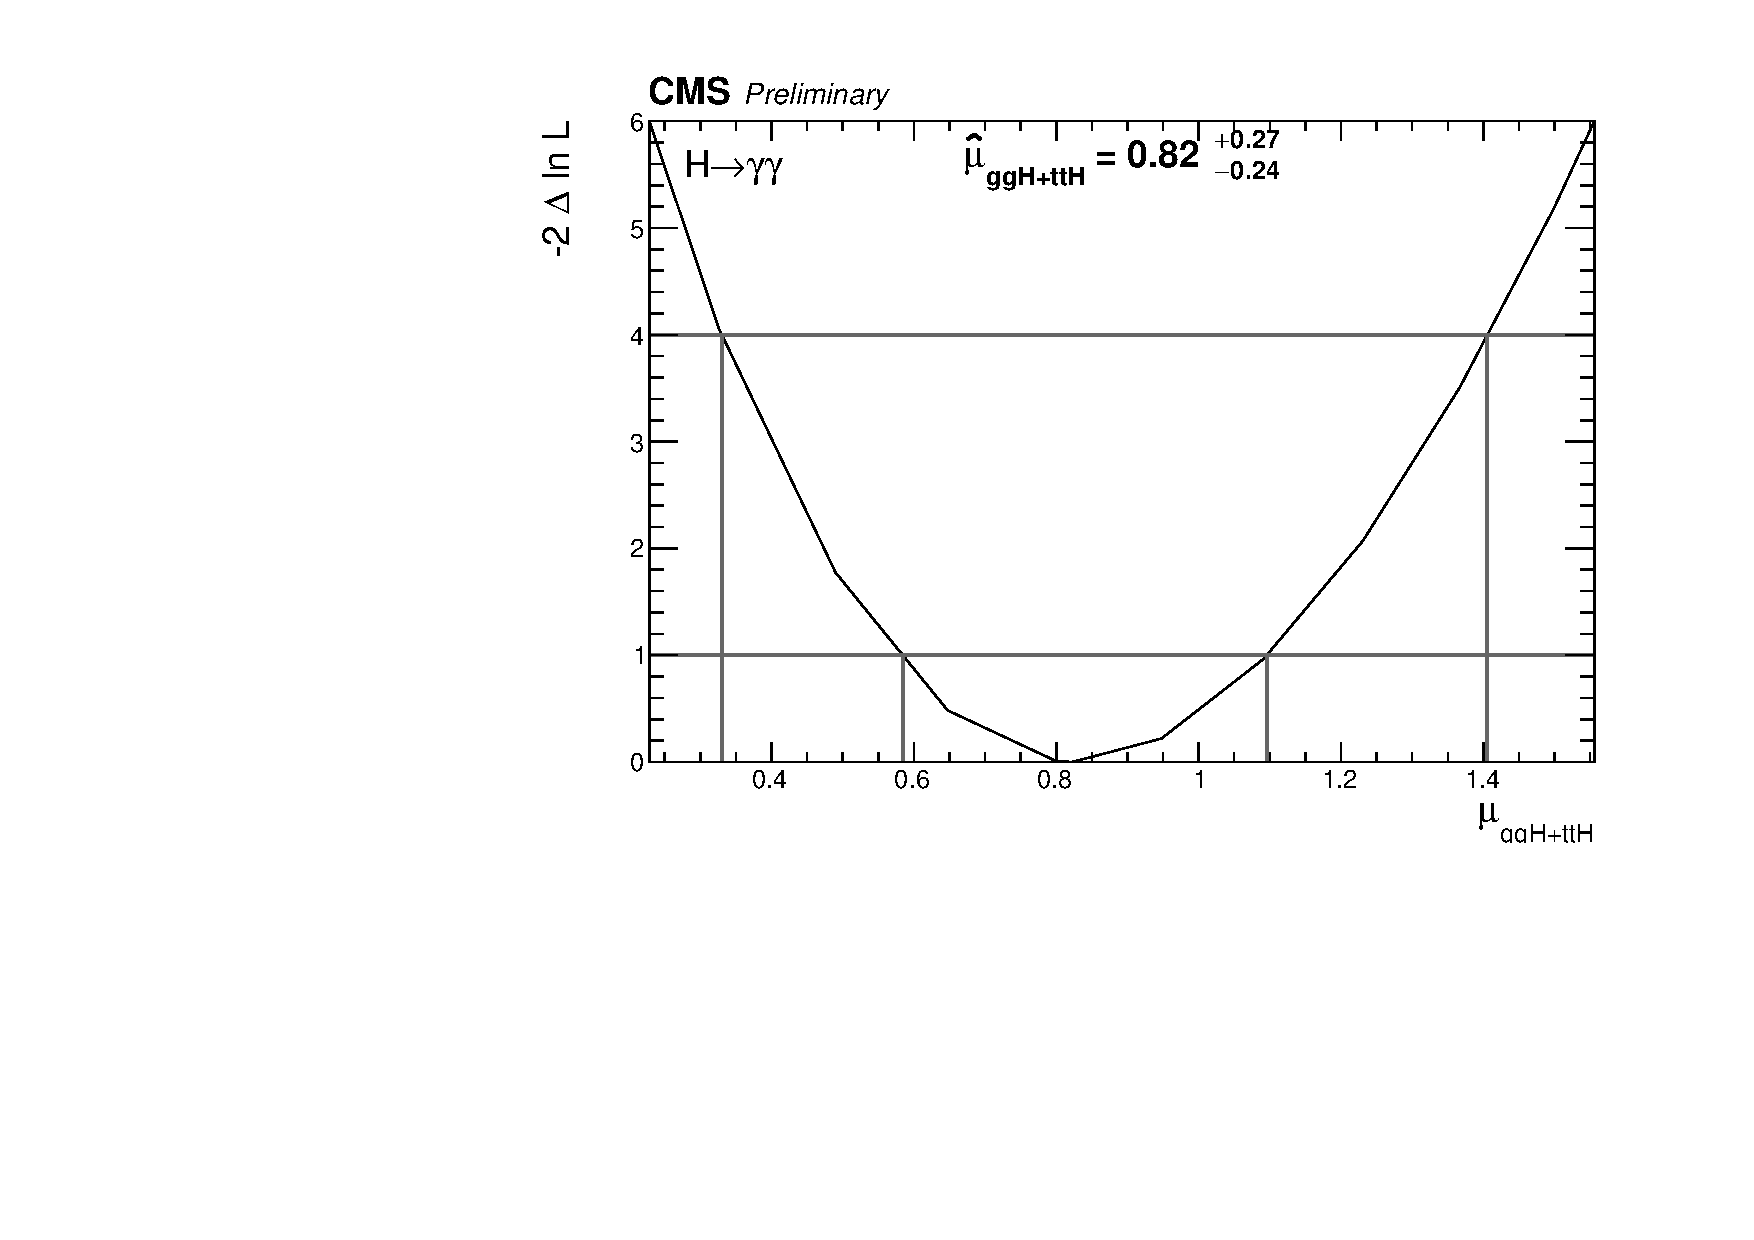
\includegraphics[width=0.83\textwidth]{statandresultsFigures/RFScanProfileMH.pdf}}
\caption{The result of performing \DNLL scans of \muF while profiling \muV (a) and vice-versa (b). In both cases the mass of the Higgs boson is profiled in the fit. }

\label{fig:statandresults:mu_per_rv_and_rf}

\end{figure}

\subsection{Per-process signal strengths}
\label{sec:statandresults:mu_per_proc}

Using a similar procedure to what was described in \Sec~\ref{sec:statandresults:rvrf}, measurements of the signal strengths of the individual Higgs boson production modes can be made. In this case, the likelihood function and test statistic are modified to contain one \POI for each production process (\muggH, \muVBF, \muVH, and \muttH). Each per-process signal strength independently scales the yield for the signal models for the corresponding process in all categories, leaving the signal models for the other processes unchanged. 

The technique described above exploits the categorisation scheme described in \Chapter~\ref{chap:categorisation}: in particular, the fact that the relative contribution from each process to the overall signal model differs from category to category. This means that varying each per-process signal strength has a different effect on the overall likelihood function. However, since no \VHTag categories are included in this analysis, it is not possible to resolve the effect of varying \muVH from other \POI\s, in particular \muggH, since most \VH events are included in the \Untagged categories along with the \ggH events. To break the degeneracy, when making the measurements of the other \POI\s, the parameter \muVH is fixed to a value of 1. 

The measurements of the \muggH, \muVBF, and \muttH are performed by producing a \DNLL scan of each parameter, while profiling the others. The \mH parameter is also profiled. The best-fit values and their uncertainties are shown on \Fig~\ref{fig:statandresults:mu_per_proc}. The measurement of the global signal strength obtained in \Sec~\ref{fig:statandresults:global_mu} is shown as the vertical black line with green bands showing the $1\sigma$ uncertainties. The \SM expectation is shown as the vertical dashed red line. The per-process signal strength measurements are all compatible with the \SM expectation within $1\sigma$. 

This result is of particular interest because certain extension to the \SM predict modified values of the per-process signal strengths. In particular, if a heavy top-like particle exists (as predicted by many theories to resolve the hierarchy problem), then an anomalous value of $\muttH$ could be observed. However, the variations in the value of \muttH predicted by such models are typically smaller than 10\%. There is evidently plenty of room to accommodate such variations in the current measurement. As more data are collected over the course of the \LHC programme, this type of measurement will become increasingly important since it could reveal clues to the nature of physics beyond the \SM, or put strong constraints on proposed extensions.

\begin{figure}[ht!]
\centering
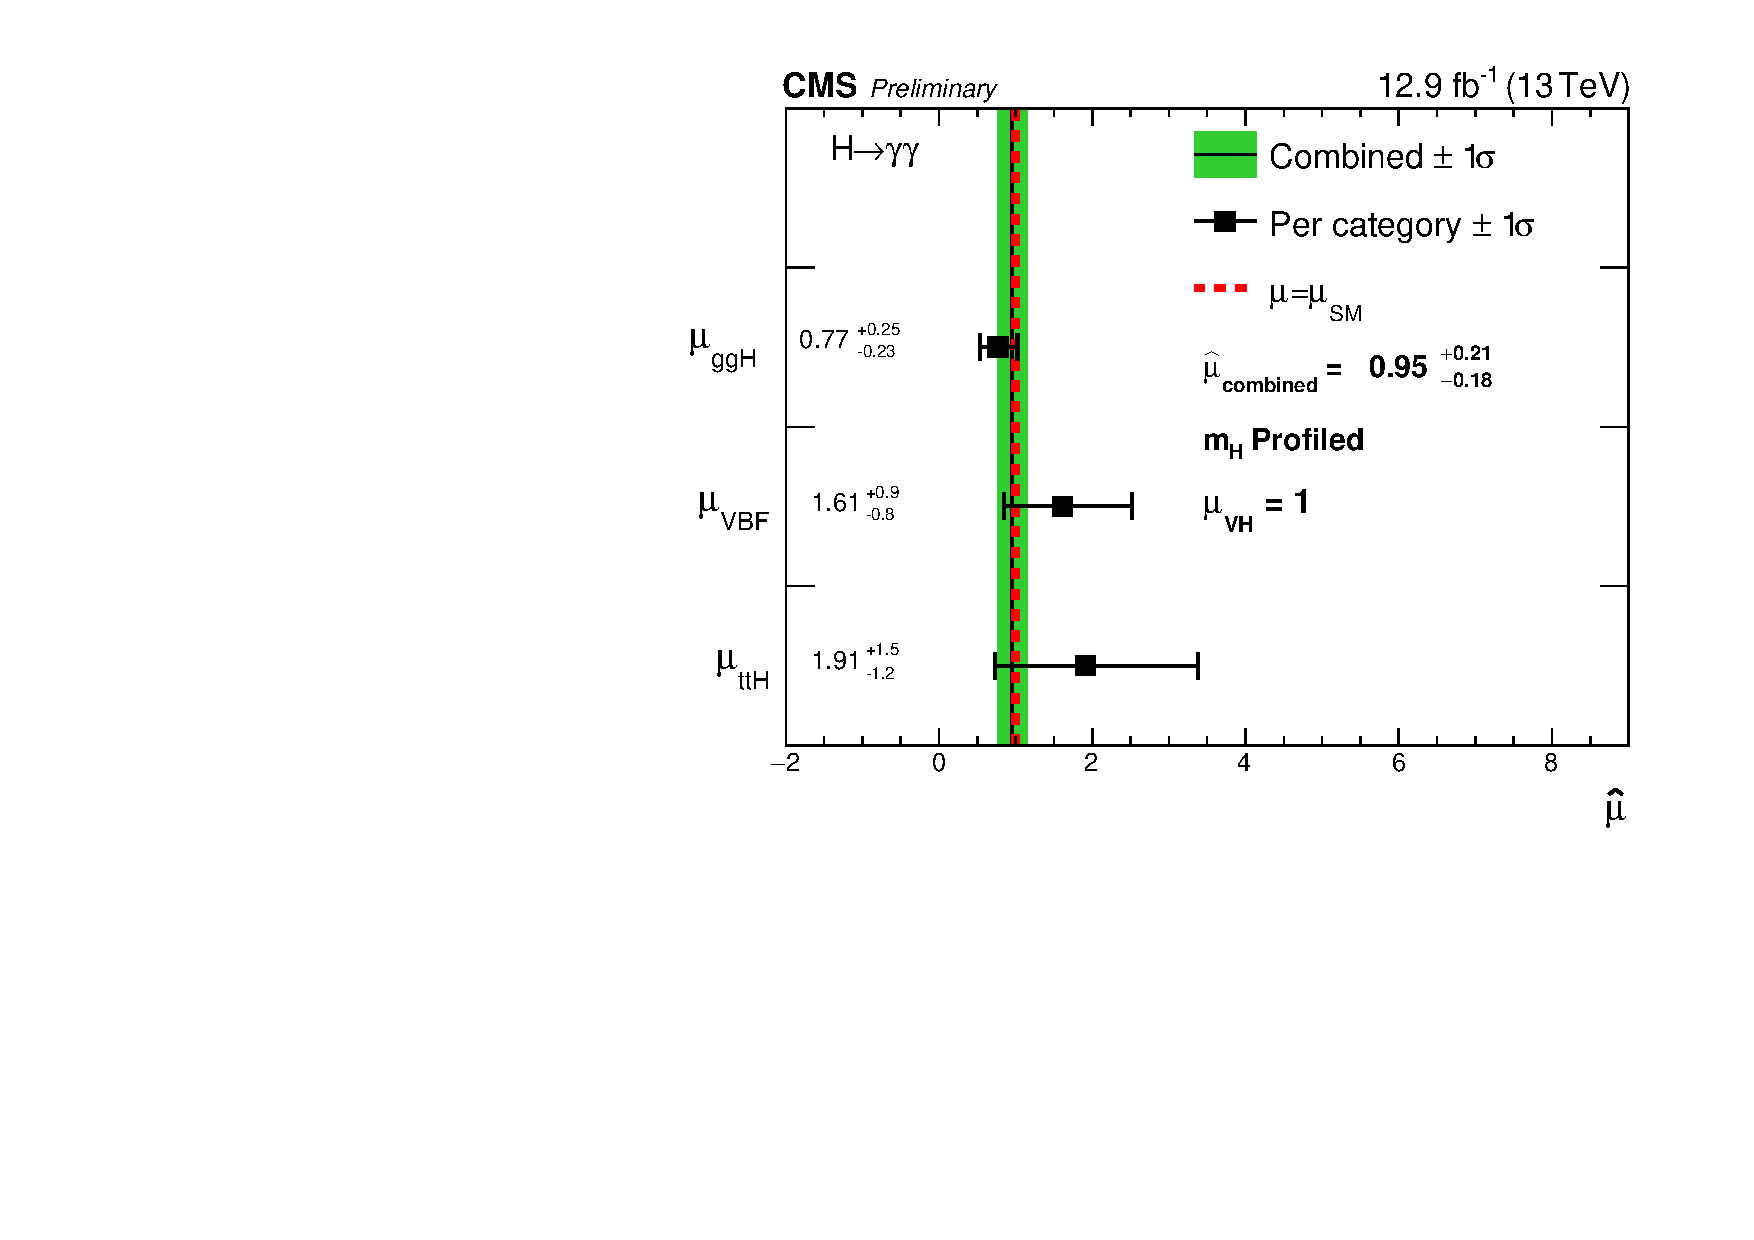
\includegraphics[width=0.95\textwidth]{statandresultsFigures/PerProcChannelCompatibilityProfileMH.pdf} 
\caption{The measurements of the per-process signal strengths \muggH, \muVBF, \muttH, obtained by performing \DNLL scans of each one while profiling the others. In each case \mH is also profiled in the fit, and $\muVH=1$ is imposed since this analysis does not include any categories specifically targeting the VH process. The vertical black line and green bands represent the measurement of the overall signal strength $\mu$, and the SM expectation is shown in the vertical red dashed line.}

\label{fig:statandresults:mu_per_proc}

\end{figure}

\subsection{Compatibility of result with SM in each category}

Using an analogous method to the one described in \Sec~\ref{sec:statandresults:mu_per_proc}, it is possible to make a measurement of the signal strength for each category separately. In this case, one \POI per analysis category is defined, which scales the yield of the signal models of all processes uniformly, but independently within each category. Although these signal strengths do not have any physical meaning, they can be used to check that each category gives a result consistent with the overall measurement, and that no bias is introduced by any particular category. The result of the check is shown in \Fig~\ref{fig:statandresults:mu_per_tag}, which determines that all the per-category signal strengths are compatible with the \SM expectation and the overall result.

\begin{figure}[ht!]
\centering
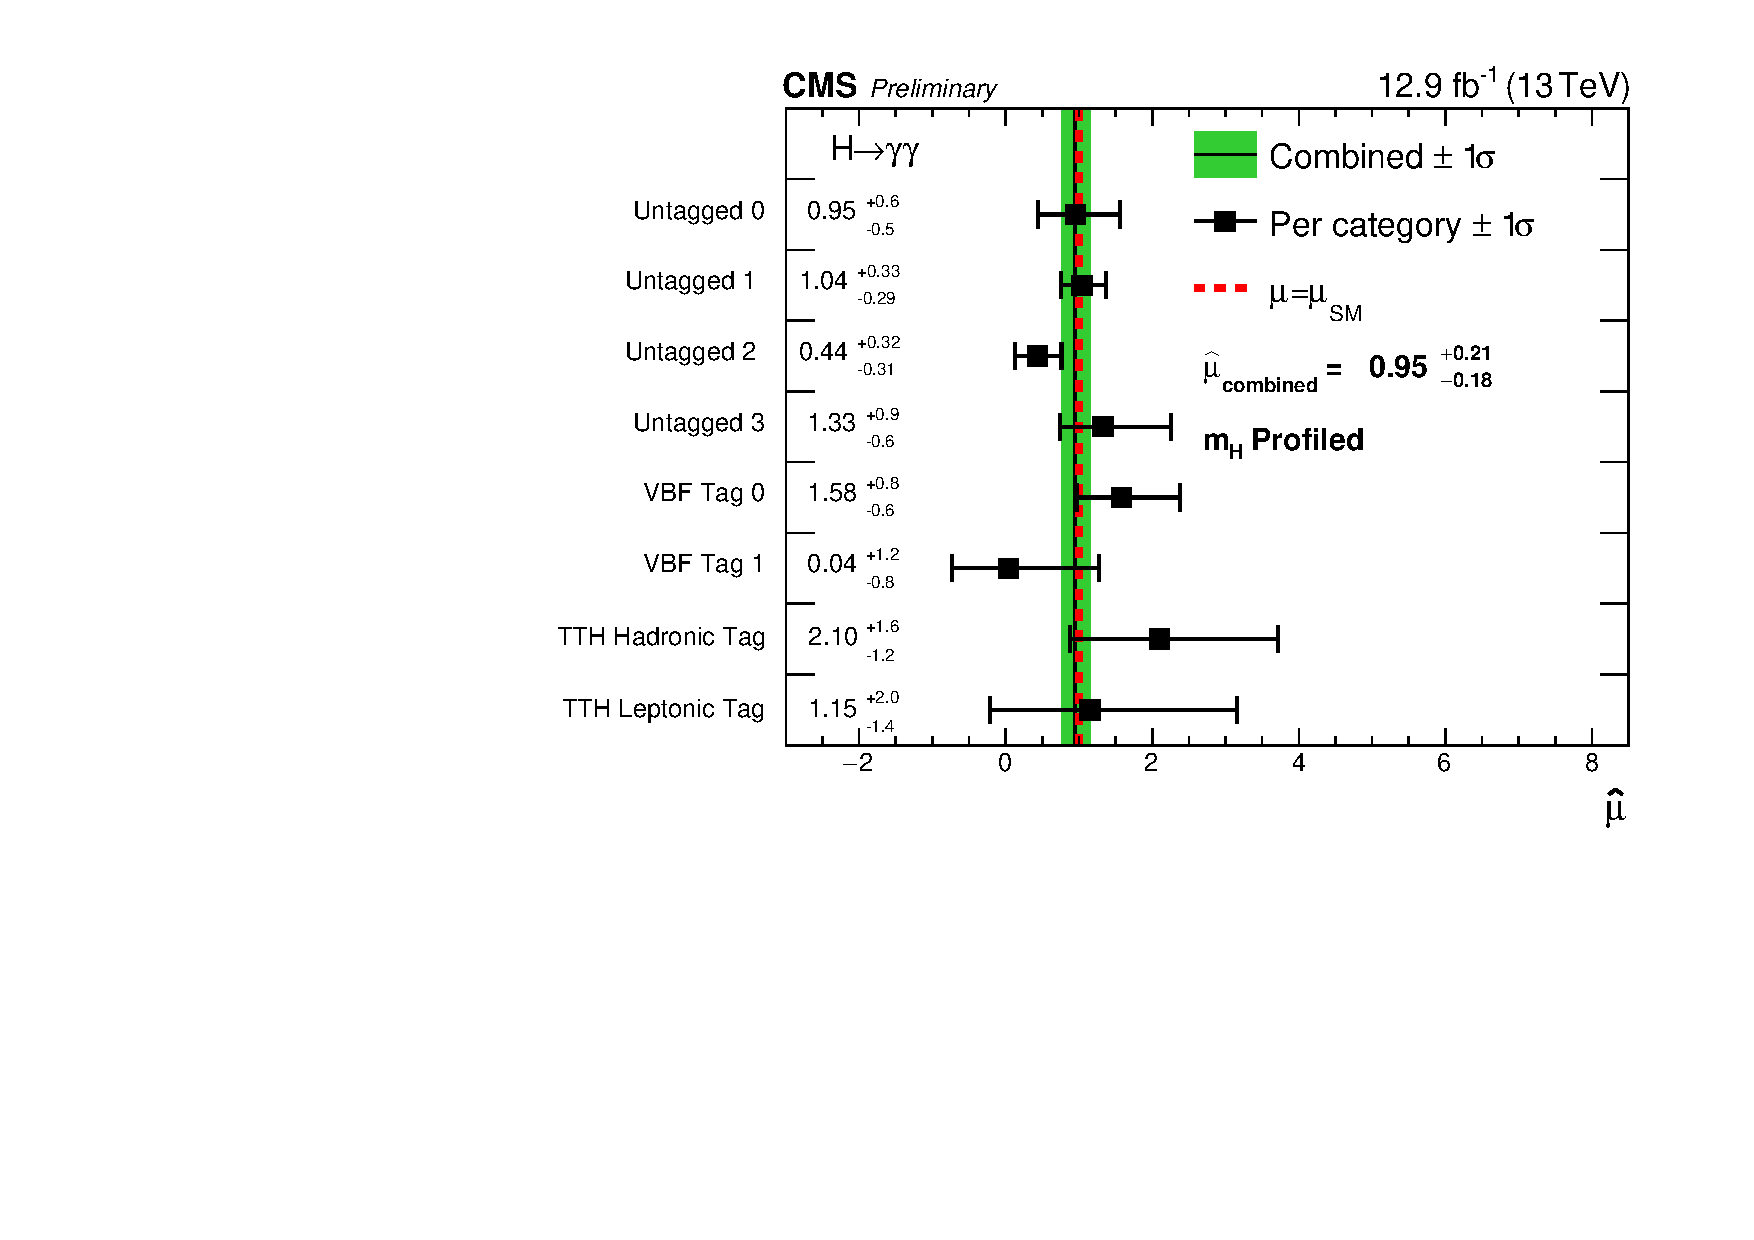
\includegraphics[width=0.95\textwidth]{statandresultsFigures/PerTagChannelCompatibilityProfileMH.pdf} 
\caption{The measurements of the per-category signal strengths, obtained by performing \DNLL scans of each one while profiling the others. In each case \mH is also profiled in the fit, The vertical black line and green bands represent the measurement of the overall signal strength $\mu$, and the SM expectation is shown in the vertical red dashed line. The per-category signal strengths are not meaningful physical observables, and this result is a check that no particular category is introducing a large bias into the overall measurement.}

\label{fig:statandresults:mu_per_tag}

\end{figure}

\section{Measurements of Higgs boson coupling modifiers}
\label{sec:statandresults:kappas}

The measurements presented so far have all dealt with Higgs boson signal strengths. Such observables are sensitive the variations in the rate at which the Higgs boson is produced, but do not take into account the possible variations in the partial width of the subsequent decay. An alternative set of measurements addresses this shortcoming by being sensitive to variations in the coupling strength of the Higgs boson with individual particles, relative to the \SM expectation. The so-called \emph{kappa} framework assigns a modifier to the coupling strength of the Higgs boson to a particle or group of particles $X$ directly in the amplitude of the process. The corresponding modifier is labelled as $\kappa_{X}$. A detailed description of the scheme is available in~\cite{Khachatryan:2016vau}.  
The assumptions which underly this framework are as follows: 
\begin{itemize}
\item any calculated deviations from the \SM are due to only one Higgs-boson-like state with mass around 125\GeV;
\item the natural width of this state is sufficiently small that it can be neglected, allowing the \crosssection and branching fraction for a process $ii\rightarrow H \rightarrow ff$ to be decomposed as $(\sigma_{ii}^{H} \cdot \Gamma_{ff}^{H}) / (\Gamma_H)$, where $\sigma_{ii}^{H}$ is the \crosssection for a Higgs boson to be produced from the initial state $ii$,  $\Gamma^{H}_{ff}$ is the partial decay width of the Higgs boson into the state $ff$ and $\Gamma_{H}$ is the total width of the Higgs boson.
\end{itemize}

The coupling modifier $\kappa_{X}$ for a particle $X$ interacting with the Higgs boson is applied directly as a factor to the corresponding $\sigma_{XX}^{H}$ if the interaction produces a Higgs boson or $\Gamma^{H}_{XX}$ if the interaction involves the decay of  a Higgs boson. For processes which only occur via loops of particles, the effective coupling modifier is defined as a function of the coupling modifiers for particles in which play a large role in the loop, e.g.~$\kappa_{\gamma} = \kappa_{\gamma}(\kappa_b, \kappa_t,\kappa_\tau,\kappa_W) $ (for the decay \Hgg) and $\kappa_{g} = \kappa_{\gamma}(\kappa_b, \kappa_t) $ (for \ggH production). 

In this measurement, coupling modifiers $\kf$ and $\kV$ are defined which uniformly scale the Higgs boson's interactions with all fermions and vector bosons respectively. The result of a two-dimensional \DNLL scan of \kf and \kV is shown in \Fig~\ref{fig:statandresults:kappa_plots_kvkf}, where the \mH parameter was profiled in the fit. The black cross indicates the best-fit while the red diamond indicates the \SM expectation. The $1\sigma$ and $2\sigma$ contours are indicated by solid and dashed lines. The best-fit indicates compatibility with the \SM. 

An interesting feature of \Fig~\ref{fig:statandresults:kappa_plots_kvkf} is that a second local minimum exists where \kf takes negative values. In general, the coupling strength modifiers always occur squared in the amplitude. However, in the \Hgg amplitude, destructive interference between the contributions of the $\Ptop$ and $\PW$ result in a term proportional to $(\kV\cdot\kf)$. This means that the measurement has a small amount of sensitivity to the sign of the coupling strength modifier $\kf$. In this measurement, the positive value is preferred, as expected by the \SM. 

%\begin{figure}[ht!]
%\centering
%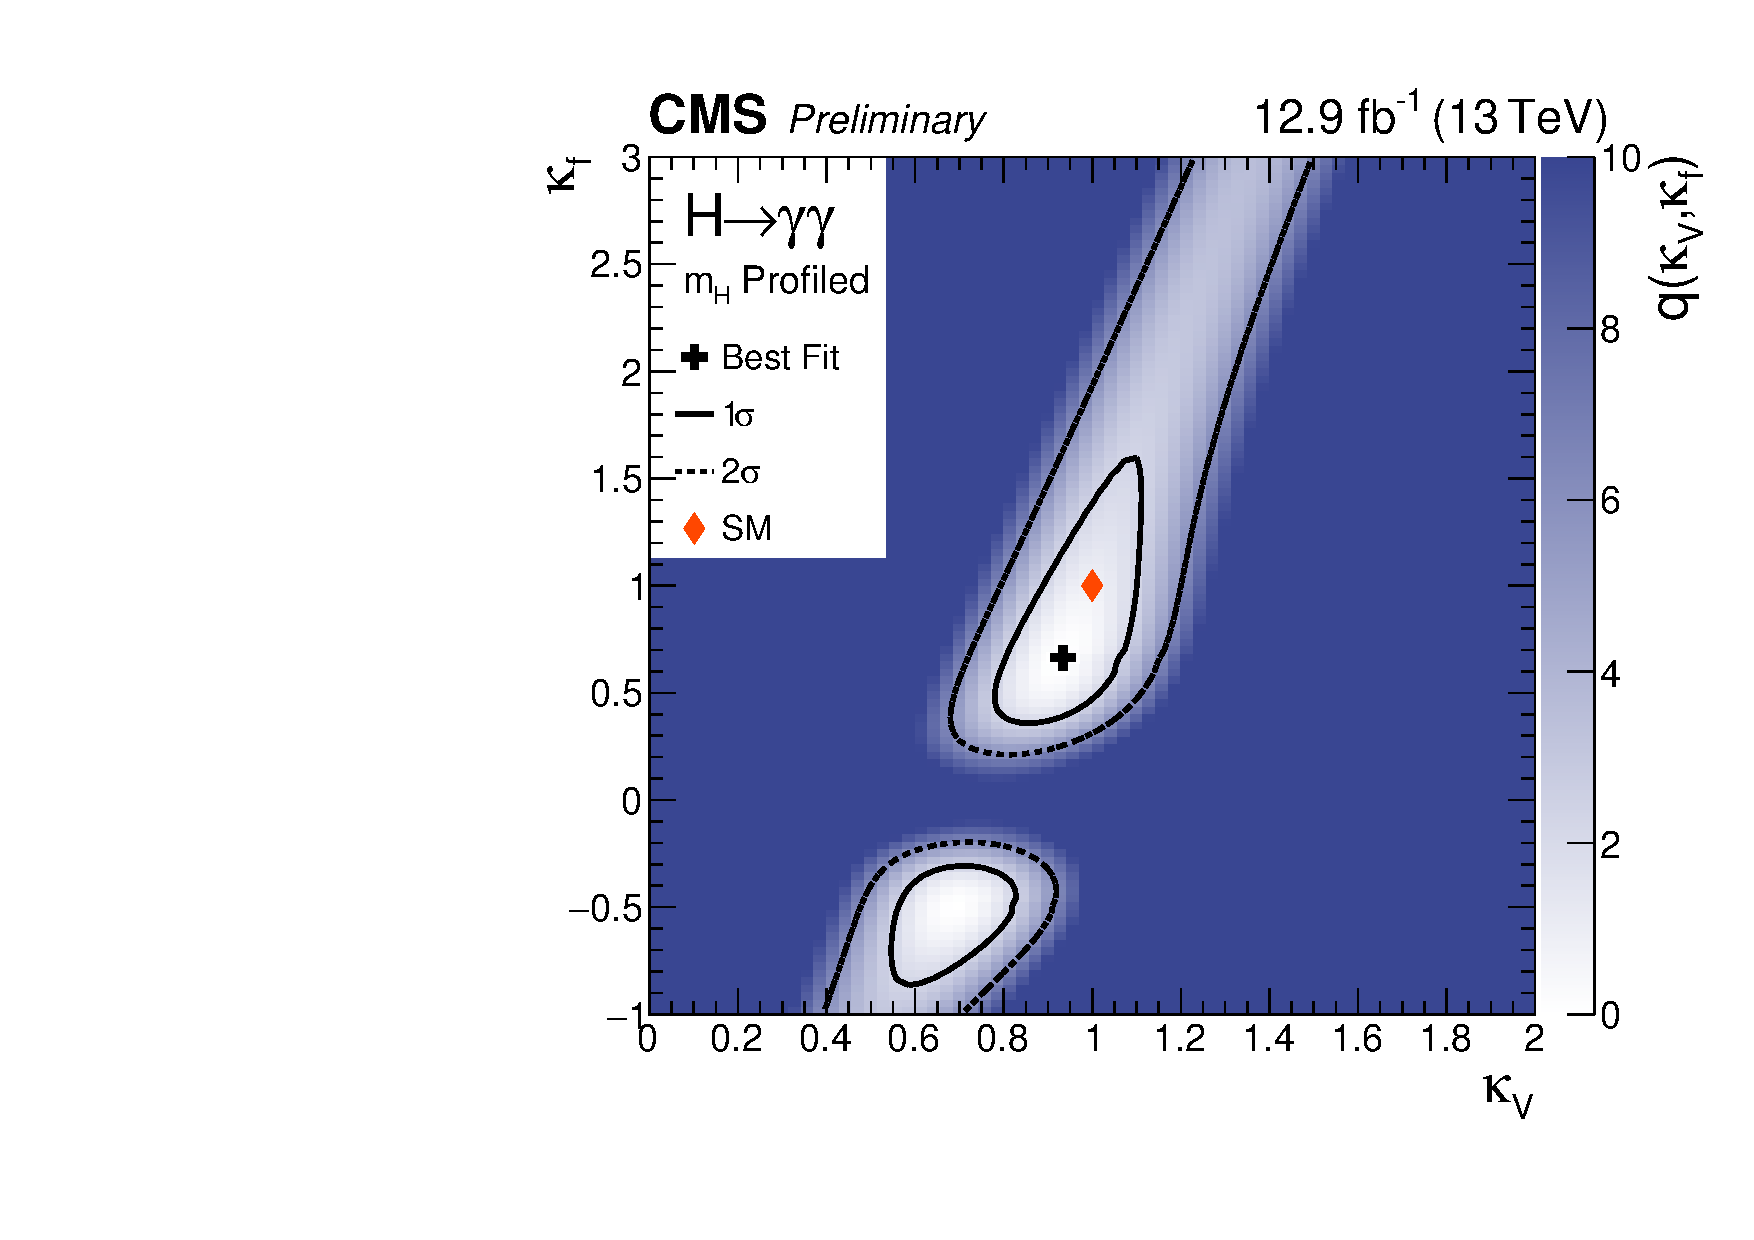
\includegraphics[width=0.6\textwidth]{statandresultsFigures/CVCFScanProfileMH_granular_col.pdf} 
%\caption{The result of a two-dimensional \DNLL scan of the coupling strength modified for fermions (\kf ) and vector bosons (\kV ). The best fit value is denoted with a black cross and the SM expected value with a red diamond. The best-fit agrees with the SM within the $1\sigma$ and $2\sigma$ uncertainty contours denoted by the solid and dashed lines respectively.}
%
%\label{fig:statandresults:kappa_plots_kvkf}
%\end{figure}

Alternatively, the measurement can be made in terms of the Higgs boson's effective coupling to gluons and photons using a two-dimensional \DNLL scan of \kGlu and \kPho, where the \mH parameter was profiled. The results are presented in \Fig~\ref{fig:statandresults:kappa_plots_kgkp}. The best-fit point agrees with the \SM within the uncertainties.


\begin{figure}[ht!]
\centering
\subfloat[\DNLL scan of \kf versus \kV]{
\label{fig:statandresults:kappa_plots_kvkf}
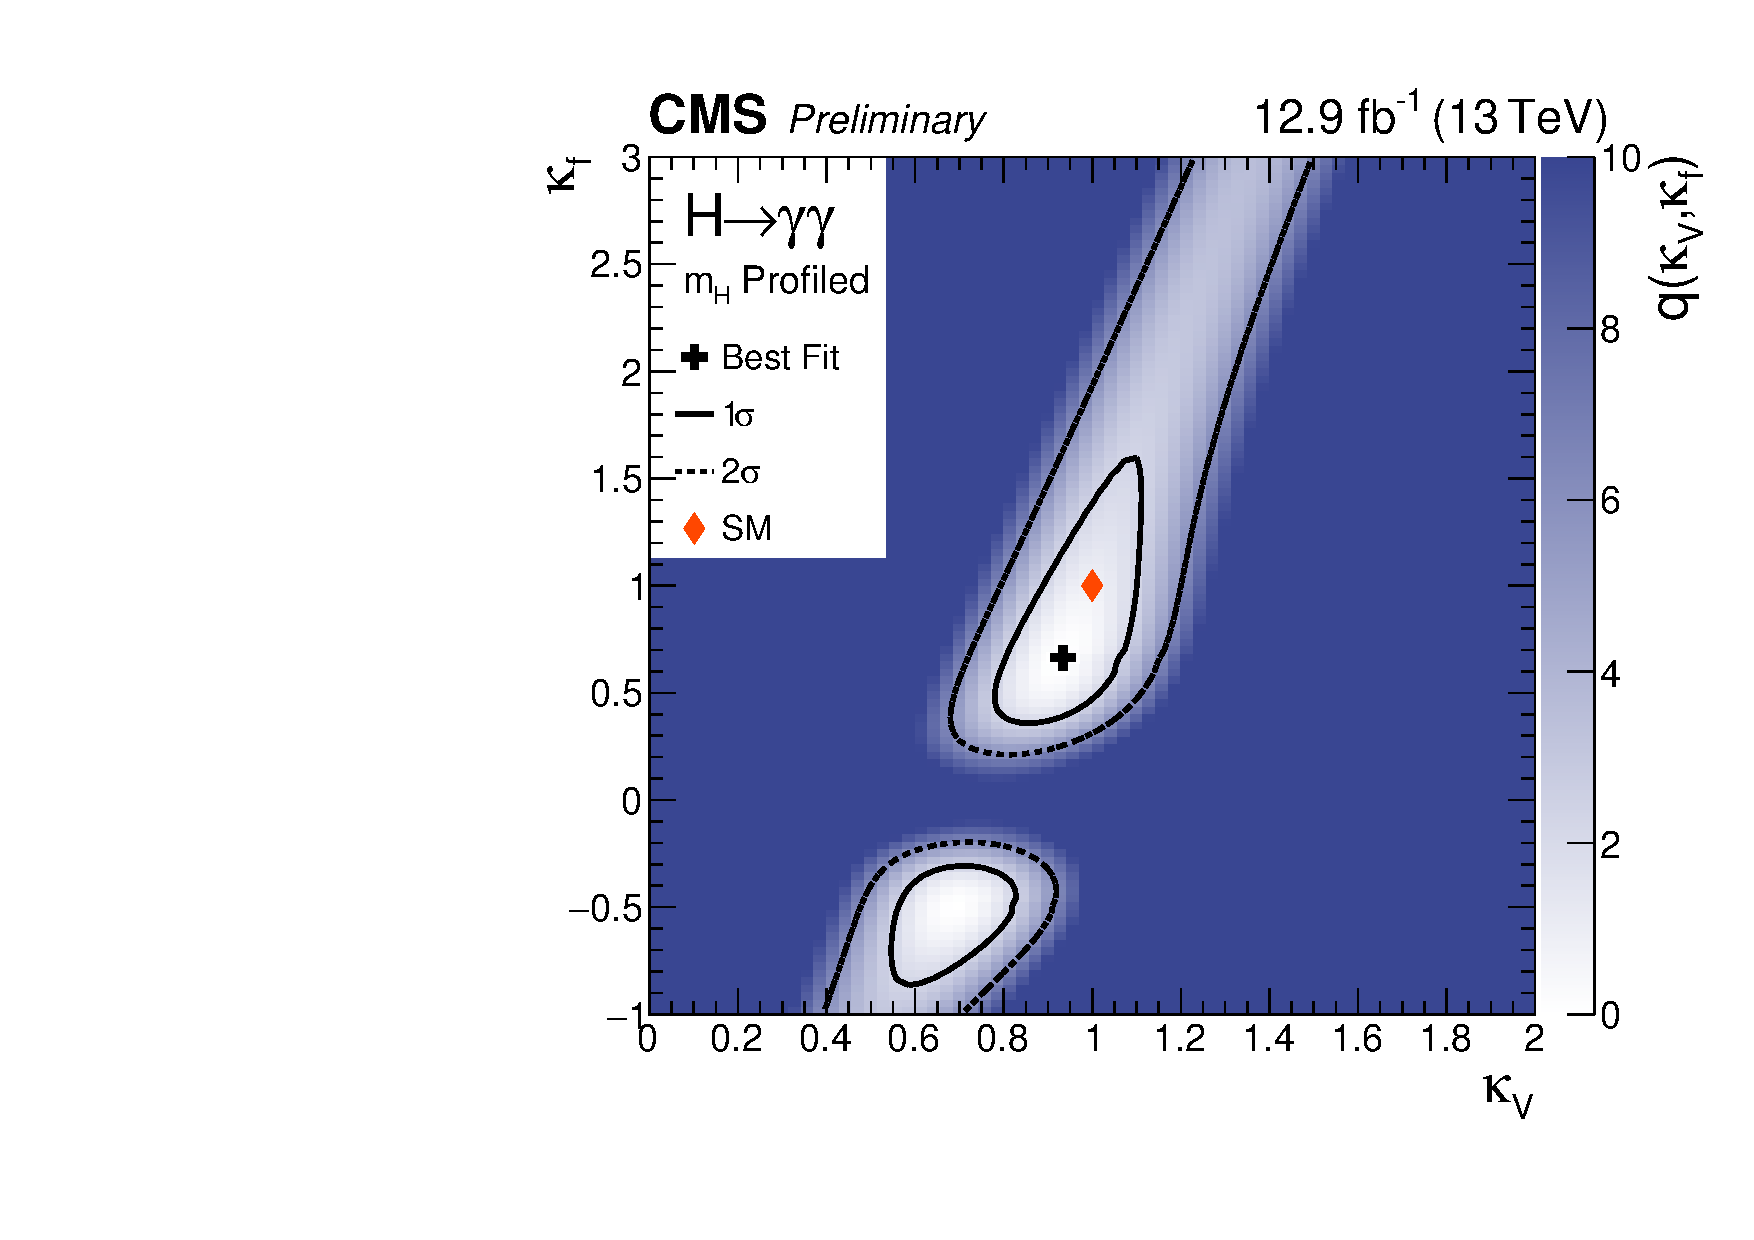
\includegraphics[width=0.65\textwidth]{statandresultsFigures/CVCFScanProfileMH_granular_col.pdf}}\\
\subfloat[\DNLL scan of \kPho versus \kGlu]{
\label{fig:statandresults:kappa_plots_kgkp}
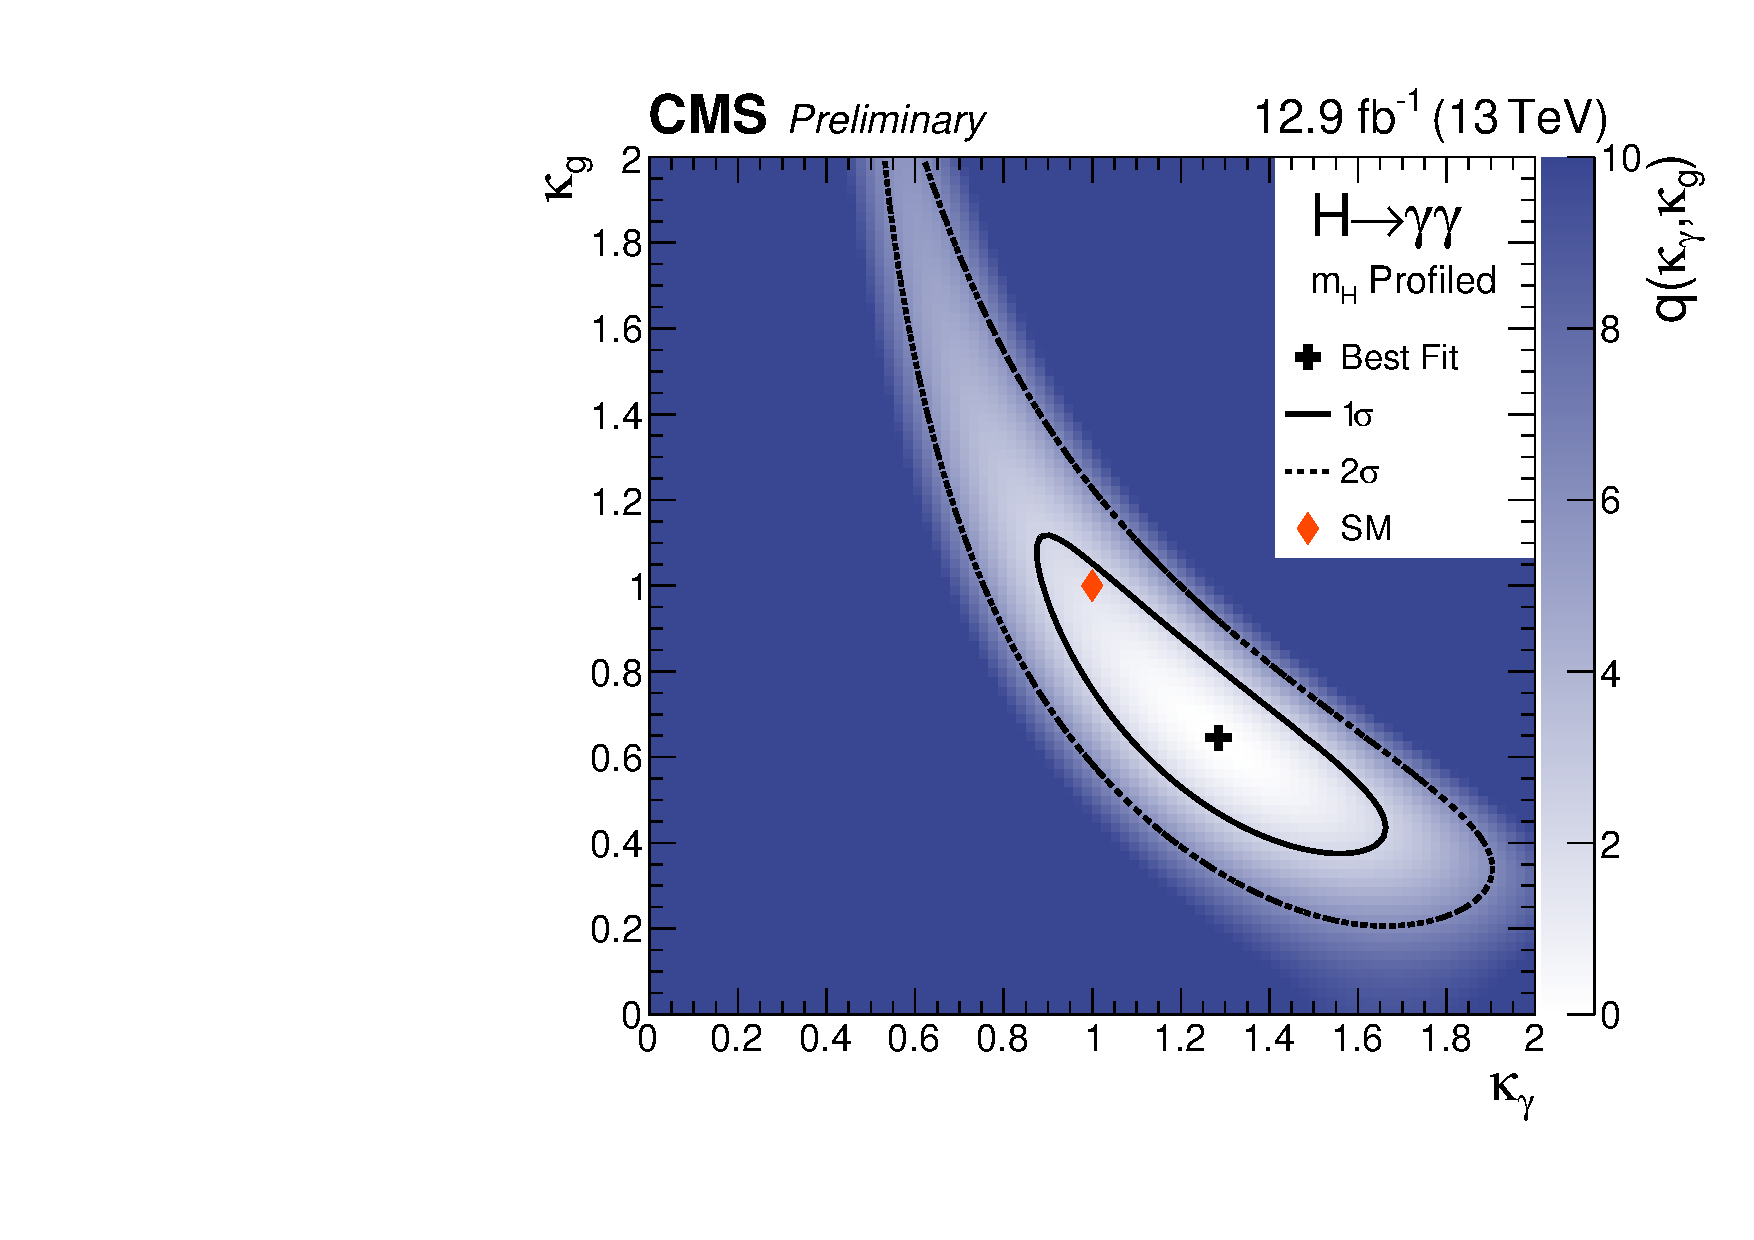
\includegraphics[width=0.65\textwidth]{statandresultsFigures/KGluKGamScanProfileMH_granular_col.pdf}}
\caption{The result of a two-dimensional \DNLL scan of the effective coupling strength modifiers for: fermions and bosons (b), and gluons and photons (b). The best-fit values are denoted with black crosses and the SM expected values with red diamonds. The best-fit points agree with the SM within the $1\sigma$ and $2\sigma$ uncertainty contours denoted by the solid and dashed lines respectively.}

\label{fig:statandresults:kappa_plots}

\end{figure}
